\documentclass{patmorin}
\listfiles
\usepackage{pat}
\usepackage{paralist}
\usepackage[OT1]{fontenc}
\usepackage[utf8]{inputenc}
\usepackage{paralist}
\usepackage{bbm}  % needed for \mathbbm{1}


\usepackage{todonotes}
\usepackage{tcolorbox}

% etoolbox allows for robust commands that don't need \protect, e.g.
% \newrobustcmd{\onesub}{\mathord{\includegraphics{figs/one-sub}}}
% \subsection{Approximate Voronoi Diagrams in $G^{\onesub}_k$}
\usepackage{etoolbox}

% david proposes the following additions
\renewcommand{\ge}{\geqslant}
\renewcommand{\le}{\leqslant}
\renewcommand{\geq}{\geqslant}
\renewcommand{\leq}{\leqslant}

\newcommand{\david}[1]{{\color{orange} David: #1}}
\newcommand{\vida}[1]{{\color{DarkGreen} Vida: #1}}
\newcommand{\pat}[1]{\textcolor{Maroon}{Pat: #1}}
\newcommand{\gwen}[1]{\textcolor{Purple}{Gwen: #1}}
\newcommand{\piotr}[1]{\textcolor{red}{Piotr: #1}}


\newenvironment{clmproof}{\noindent\emph{Proof of Claim:}}{\hfill\rule{1ex}{1ex}}

\usepackage[longnamesfirst,numbers,sort&compress]{natbib}

\usepackage[mathlines]{lineno}
\setlength{\linenumbersep}{2em}
% \linenumbers
% \rightlinenumbers
% \linenumbers
\newcommand*\patchAmsMathEnvironmentForLineno[1]{%
 \expandafter\let\csname old#1\expandafter\endcsname\csname #1\endcsname
 \expandafter\let\csname oldend#1\expandafter\endcsname\csname end#1\endcsname
 \renewenvironment{#1}%
    {\linenomath\csname old#1\endcsname}%
    {\csname oldend#1\endcsname\endlinenomath}}%
\newcommand*\patchBothAmsMathEnvironmentsForLineno[1]{%
 \patchAmsMathEnvironmentForLineno{#1}%
 \patchAmsMathEnvironmentForLineno{#1*}}%
\AtBeginDocument{%
\patchBothAmsMathEnvironmentsForLineno{equation}%
\patchBothAmsMathEnvironmentsForLineno{align}%
\patchBothAmsMathEnvironmentsForLineno{flalign}%
\patchBothAmsMathEnvironmentsForLineno{alignat}%
\patchBothAmsMathEnvironmentsForLineno{gather}%
\patchBothAmsMathEnvironmentsForLineno{multline}%
}



% Taken from
% https://tex.stackexchange.com/questions/42726/align-but-show-one-equation-number-at-the-end
\newcommand\numberthis{\addtocounter{equation}{1}\tag{\theequation}}

\definecolor{brightmaroon}{rgb}{0.76, 0.13, 0.28}
\definecolor{linkblue}{rgb}{0, 0.337, 0.227}
\newcommand{\defin}[1]{\emph{\textcolor{brightmaroon}{#1}}}
\makeatletter
\def\mathcolor#1#{\@mathcolor{#1}}
\def\@mathcolor#1#2#3{%
  \protect\leavevmode
  \begingroup
    \color#1{#2}#3%
  \endgroup
}
\makeatother
\newcommand{\mathdefin}[1]{\mathcolor{brightmaroon}{#1}}
% \newcommand{\mathdefin}[1]{\color{brightmaroon}#1}}
\setlength{\parskip}{1ex}

% Document-specific commands and math operators
\DeclareMathOperator{\tw}{tw}
\DeclareMathOperator{\pw}{pw}
\DeclareMathOperator{\bw}{bw}
\DeclareMathOperator{\ld}{ld}
\DeclareMathOperator{\polylog}{polylog}
\DeclareMathOperator{\evol}{Evol}
\DeclareMathOperator{\ivol}{Ivol}
\DeclareMathOperator{\tvol}{Tvol}


\title{\MakeUppercase{Fan-Partitions of Planar Graphs (and Beyond)
  \newline by Local Sparsification and Volume-Preserving Embeddings}}
\author{TBD}

% \author{
% Vida Dujmovi{\'c}\,\footnotemark[6]\qquad
% Gwena\"el Joret\,\footnotemark[4] \qquad
% Piotr Micek\,\footnotemark[5] \\
% Pat Morin\,\footnotemark[9]\qquad
% David~R.~Wood\,\footnotemark[2]
% }

% \footnotetext[2]{School of Mathematics, Monash University, Melbourne, Australia (\texttt{david.wood@monash.edu}). Research of Wood supported by the Australian Research Council.}

% \footnotetext[6]{School of Computer Science and Electrical Engineering, University of Ottawa, Ottawa, Canada (\texttt{vida.dujmovic@uottawa.ca}). Research supported by NSERC.}

% \footnotetext[4]{D\'epartement d'Informatique, Universit\'e libre de Bruxelles, Belgium (\texttt{\{gwenael.joret,michal.seweryn\}@ulb.be}). G.\ Joret is supported by a CDR grant from the Belgian National Fund for Scientific Research (FNRS), by a PDR grant from FNRS, and by the Australian Research Council.}

% \footnotetext[5]{Department of Theoretical Computer Science, Jagiellonian University, Kraków, Poland (\texttt{piotr.micek@uj.edu.pl}). Research supported
% the National Science Center of Poland under grant UMO-2018/31/G/ST1/03718 within the BEETHOVEN program.}

% \footnotetext[9]{School of Computer Science, Carleton University, Ottawa, Canada (\texttt{morin@scs.carleton.ca}). Research supported by NSERC and the Ontario Ministry of Research and Innovation.}


\date{}


\begin{document}

\maketitle

\begin{abstract}
  We show that every $n$-vertex planar graph is contained in the strong product of a fan and a clique of size $O(\sqrt{n}\log^2 n)$.  Equivalently, every $n$-vertex planar graph $G$ contains a vertex subset $X$ of size $O(\sqrt{n}\log^2 n)$ such that $G-X$ has bandwidth $O(\sqrt{n}\log^2 n)$.  This result holds in the more general setting of product structured graphs, which includes bounded genus graphs and $k$-planar graphs for fixed $k$.
\end{abstract}

\section{Introduction}


The \defin{$k$-blowup} of a graph $H$ is the graph obtained by replacing each vertex $v$ of $H$ with a clique $K_v$ of size $k$ and replacing each edge $vw$ of $H$ with a complete bipartite graph with parts $V(K_v)$ and $V(K_w)$.  The current work is motivated by the following question: What is the simplest family of graphs $\mathcal{H}$ such that for each $n$-vertex planar graph $G$ there is a graph $H\in\mathcal{H}$ such that $G$ is contained in a $\tilde{O}(\sqrt{n})$-blowup of $H$\david{, where $\tilde{O}$ notation hides $\polylog(n)$ terms}?\footnote{We say that a graph $G$ is \defin{contained} in a graph $G'$ if \david{$G$ is isomorphic to a subgraph of $G'$} $G'$ contains a subgraph isomorphic to $G$.}

\citet{ISW} show that one can take $\mathcal{H}$ to be the class of treewidth-$3$ graphs. \citet{distel.dujmovic.ea:product} show that even \david{delete `even'} the class of treewidth-$2$ graphs is sufficient.  In the current work, we show that one can even take $\mathcal{H}$ to be the class of pathwidth-$2$ graphs.  Even more specifically, every $n$-vertex planar graph is isomorphic to a $\tilde{O}(\sqrt{n})$-blowup of a fan.\footnote{A \defin{fan} $F_k$ is a graph with \david{$V(F_k):=\{v_0,\ldots,v_k\}$ and $E(F_k):=\{v_0v_i:1\leq i\leq k\}\cup\{v_iv_{i+1}:1\leq i\leq k-1\}$} vertex set $V(F_k):=\{v_0,\ldots,v_k\}$ whose edge set consists of a path on $v_1,\ldots,v_k$ and an edge from $v_0$ to each of $v_1,\ldots,v_k$.}

\begin{thm}\label{main_thm_planar}
  For every $n$-vertex planar $G$ there is a $O(\sqrt{n}\log^2 n)$-blowup of a fan that contains a subgraph isomorphic to $G$.
\david{Rephrase: Every $n$-vertex planar graph is contained in a $O(\sqrt{n}\log^2 n)$-blowup of a fan.}
\end{thm}

\david{At this point we should acknowledge (at least in a footnote) that the previous results had no $\polylog(n)$ term in the blowup, otherwise the referee will rightly acuse us of being misleading. }

The choice of parameter $\sqrt{n}$ in these results is not arbitrary. A $k$-blowup of a treewidth-$t$ graph $H$ has treewidth \david{at most} $k(t+1)-1$.  Since there $n$-vertex planar graphs of treewidth $\Omega(\sqrt{n})$ \david{(such as the $\sqrt{n}\times\sqrt{n}$ grid)}, any result like \cref{main_thm_planar} that finds all planar graphs in blowups of bounded treewidth graphs must have blowups of size $\Omega(\sqrt{n})$.  Pathwidth $2$ is is also the best-possible bound in theorems like  \cref{main_thm_planar}.  Indeed, even \emph{treewidth} $1$ is not achievable:  The fan $F_n$ is not contained in $k$-blowup of a tree for any $k\in o(n)$ \david{This is false. $F_n$ is contained in the $\sqrt{n}$ blowup of the $\sqrt{n}$-leaf star. Instead write ``\citet{LMST08} describe an infinite family of $n$-vertex planar graphs $G$ such that every (improper) 2-colouring has a monochromatic component on $\Omega(n^{2/3})$ vertices. Say $G$ is contained in a $k$-blowup $(K_v:v\in V(T))$ of a tree $T$. Colour each vertex in each $K_v$ by the colour of $v$ in a proper 2-colouring of $T$. So each monochromatic compononent is contained in some $K_v$, implying that $k\in\Omega(n^{2/3})$. }.

\david{Stuff to add to the intro:
\begin{itemize}
    \item $O(\sqrt{n})$ blowups imply and strengthen the Lipton--Tarjan separator theorem. Without this, the naive reader will ask ``what is the point?''
\item \citet{distel.dujmovic.ea:product} asked whether every $n$-vertex planar graph is contained in a $O(\sqrt{n})$-blowup of a graph with bounded pathwidth. \cref{main_thm_planar} shows the answer is ``yes'' with $O(\sqrt{n})$ replaced by $\tilde{O}(\sqrt{n})$.
\item Results of \citet[Theorem~5]{DvoWoo} imply that for all $\epsilon>0$ there exists $c$ such that every $n$-vertex planar graph is contained in a $O(n^{1/2+\epsilon})$-blowup of a graph $H$ with treedepth $c$, which implies $\pw(H)\leq c-1$. \citet[Theorem~19]{DvoWoo} also establish a corresponding lower bound: for any $c\geq 1$ there exists $\epsilon>0$ such that if the $\sqrt{n}\times\sqrt{n}$ grid is contains in a $k$-blowup of a graph $H$ with treedepth at most $c$, then $k\geq\Omega(n^{1/2+\epsilon})$. (In fact, these lower and upper bounds match.)\ Thus the $\sqrt{n}\times \sqrt{n}$-grid is not contained in a $\tilde{O}(n^{1/2})$-blowup of a graph with bounded treedepth. In this sense, the `bounded pathwidth' condition in \cref{main_thm_planar} is best posible.
\end{itemize}}



\subsection{Product Structured Graphs}

\cref{main_thm_planar} follows from a more general theorem about subgraphs of certain strong graph products, as we now explain.  The \defin{strong product} $A\boxtimes B$ of two graphs $A$ and $B$ is the graph with vertex set $V(A\boxtimes B):=V(A)\times V(B)$ that contains an edge with endpoints $(v_1,v_2)$ if and $(w_1,w_2)$ if and only if
\begin{compactenum}
    \item $v_1w_1\in E(A)$ and $v_2=w_2$;
    \item $v_1=w_1$ and $v_2w_2\in E(B)$; or
    \item $v_1w_1\in E(A)$ and $v_2w_2\in E(B)$.
\end{compactenum}
Note that $k$-blowup of $H$ can be written as the strong product $H\boxtimes K_k$.  Therefore, \cref{main_thm_planar} states that, for every $n$-vertex planar graph $G$ there is a fan $F$ such that $G$ is isomorphic to a subgraph of $F\boxtimes K_{O(\sqrt{n}\log^2 n)}$. \david{We prove the following more general result.}

\begin{thm}\label{main_thm_products}
  For every graph $H$ with treewidth $t$, for every path $P$, and for every $n$-vertex subgraph $G$ of $H\boxtimes P$ there is a $O(t\sqrt{n}\log^2 n)$-blowup of a fan that contains a subgraph isomorphic to $G$.
  \david{rephrase: every $n$-vertex subgraph of $H\boxtimes P$ is contained in a $O(t\sqrt{n}\log^2 n)$-blowup of a fan.}
\end{thm}

\Cref{main_thm_products} implies \cref{main_thm_planar} by the following \defin{Planar \david{Graph} Product Structure Theorem}:

\begin{thm}[\cite{dujmovic.joret.ea:planar,ueckerdt.wood.ea:improved}]\label{planar_product_structure}
  For every planar graph $G$, there exists a graph $H$ of treewidth $6$ and a path $P$ such $G$ is isomorphic to a subgraph of $H\boxtimes P$.
\end{thm}

\Cref{planar_product_structure} has been generalized to a number of other minor-closed and non-minor closed graph classes, including bounded genus graphs and (more generally) apex-minor-free graphs \cite{dujmovic.joret.ea:planar,distel.hickingbotham.ea:improved} and $k$-planar graphs \cite{dujmovic.morin.ea:graph,distel.hickingbotham.ea:powers}.

\pat{TODO: Write a corollary of \cref{main_thm_products} that lists some of the graph classes with product structure.} \david{here is an attempt}

\cref{main_thm_planar} generalises for graphs embeddable on arbitrary surfaces as follows. The \defin{Euler genus} of a surface with $h$ handles and $c$ crosscaps is $2h+c$. The \defin{Euler genus} of a graph $G$ is the minimum Euler genus of a surface in which $G$ embeds without crossings.
Building on previous work in \citep{dujmovic.joret.ea:planar,ueckerdt.wood.ea:improved}, \citet{distel.hickingbotham.ea:improved} showed that every graph $G$ of Euler genus $g$ is contained in $H\boxtimes P$ for some graph $H$ with treewidth $2g+6$ and for some path $P$. \cref{main_thm_products} thus implies:

\begin{thm}\label{genus_products}
Every $n$-vertex graph of Euler genus $g$ is contained in a $O((g+1)\sqrt{n}\log^2 n)$-blowup of a fan.
\end{thm}

We have the following further generalisation.
A graph $X$ is \defin{apex} if $X-a$ is planar for some vertex $a\in V(X)$. \citet{dujmovic.joret.ea:planar} showed that for every apex graph $X$ there exists $c$ such that every $X$-minor-free graph is contained in $H\boxtimes P$ for some graph $H$ with treewidth $c$ and for some path $P$ (and such a theorem holds only if $X$ is apex). \cref{main_thm_products} thus implies:

\begin{thm}\label{apex_products}
For every fixed apex graph $X$, every $n$-vertex $X$-minor-free graph is contained in a $O(\sqrt{n}\log^2 n)$-blowup of a fan.
\end{thm}

Product structure theorems are known for various non-minor-closed classes~\citep{dujmovic.morin.ea:graph,HW24,distel.hickingbotham.ea:powers}. For example, a graph is \defin{$(g,k)$-planar} if it has a drawing in a surface of Euler genus $g$ with at most $k$ crossings on each edge. \citet{dujmovic.morin.ea:graph} proved that every $(g,k)$-planar graph is contained in $H\boxtimes P$ for some graph $H$ with treewdth $O((g+1)k^5)$ and for some path $P$.

\cref{main_thm_products} thus implies:

\begin{thm}\label{gkplanar_products}
Every $n$-vertex $(g,k)$-planar graph is contained in a $O((g+1)k^5\sqrt{n}\log^2 n)$-blowup of a fan.
\end{thm}

\david{
Do we get improved depedennce working with subgraph of $H\boxtimes P \boxtimes K_c$? (e.g. for $k$-planar graphs we can use $\tw(H)=10^{10}$ and $c=c_k$).
}

\pat{Now I can answer the question: No, the bound will be $O(tc\sqrt{n}\log^2 n)$.  The bottleneck is the sparsification lemma.  The size of the set $X$ there becomes $O((t+1)c(n/D)\log n)$.  Interestingly (maybe) when $G$ is a subgraph of $H\boxtimes P\boxtimes K_c$, the metric space $(V(G),d_{H\boxtimes P\boxtimes K_c})$ has $(k,O(t\sqrt{\log n}))$-volume-respecting embeddings, for any $c$. If you take $t=0$ and $c=n$ then you get a metric space where $d(v,w)=1$ for all  $v,w\in V(G)$ and this has as $(k,O(\sqrt{\log n}))$-volume respecting embedding.  The proof of this is much simpler: Every vertex maps to a uniformly random point in a $O(k\log n)$-dimensional ball of diameter $1$ (so the radius of the ball is $O(1/\sqrt{k\log n}))$.  Then the proof ``just'' boils down to showing that, with probability at least $1-n^{-ck}$, $k$ random points in this ball define a $(k-1)$-simplex whose $(k-1)$-dimensional volume is $\Omega((1/((k-1)!\sqrt{\log n})^{k-1}))$. \\[2ex]
We should somehow get this point across in the introduction:  The metric space $(V(G),d_G)$ is awkward to work with directly for the same reason that planar graphs are awkward to work with directly; it's hard to see any structure.  The metric space $(V(G),d_{K_n})$ is a contraction of $(V(G),d_G)$ which makes it suitable to work with, and it's highly regular, but it's too ``dense'' to have any useful properties.  The metric space $(V(G),d_{H\boxtimes P})$ is a perfect middle-ground; it's highly regular (like $(V(G),d_{K_n}))$ but ``sparse'' enough to admit a local sparsification lemma \david{include this paragraph as is}.\\[2ex]
It might be a useful exercise to find what properties of a metric space are sufficient to prove a local sparsification lemma.  Here's a first try:\\[2ex]
Let $(S,d)$ be a finite metric space, let $L_0\subseteq S$, and for each $0\le a\le b$, let $L_{[a,b]}:=\{x\in S: a\le d(x,L_0)\le b\}$.  Now I'm stuck.  There is no obvious notion of a set $X\subseteq S$ that separates two subsets $A,B$ of $S$.
}

\subsection{Relation to Bandwidth}

An \defin{$H$-partition} of a graph $G$ is a partition $\mathcal{P}:=\{B_x: x\in V(H)\}$ of $V(G)$ whose parts are indexed by the vertices of $H$ such that, for each edge $vw$ of $G$, $v$ and $w$ are in the same part or there exists an edge $xy$ of $H$ such that $v\in B_x$ and $w\in B_y$.  The \defin{width} of $\mathcal{P}$ is the maximum size of any part.  It follows immediately from this definition that $G$ has an $H$-partition of width $w$ if and only if $G$ is isomorphic to a subgraph of $H\boxtimes K_w$. When $H$ is a member of some class $\mathcal{H}$ of graphs, we call an $H$-partition of $G$ an \defin{$\mathcal{H}$-partition} of $G$.  For example, if $H$ is path, tree, or fan, then we call an $H$-partition a path-partition, a tree-partition, or a fan-partition, respectively.  The \defin{$\mathcal{H}$ partition width}  of a graph $G$ is the minimum integer $w$ such that $G$ has an $\mathcal{H}$-partition of width $w$. Thus, \cref{main_thm_planar} states that every $n$-vertex planar graph has fan partition width
\david{Hyphenate $\mathcal{H}$-partition-width, fan-partition, fan-partition-width, path-partition, path-partition-width throughout}
$O(\sqrt{n}\log^2 n)$.

\david{in the context of bandwidth, `ordering' is used instead of `permutation'}
Let $G$ be a graph and let $v_1,\ldots,v_n$ be a permutation of $V(G)$.  Then $v_1,\ldots,v_n$ has \defin{bandwidth} $\mathdefin{\bw_G(v_1,\ldots,v_n)}:=\{\max\{j-i: v_iv_j\in E(G)\}$
\david{$|j-i|$}.  The \defin{bandwidth} of $G$ is $\mathdefin{\bw(G)}:=\min\{\bw_G(v_1,\ldots,v_n):\text{$v_1,\ldots,v_n$ is a permutation of $V(G)$}\}$. The bandwidth of a graph $G$ is closely related to the path partition width of $G$.  Indeed, if $\bw_G(v_1,\ldots,v_n)=w$, and $P:=x_1,\ldots,x_{\lceil n/w\rceil}$ is a path, then setting $B_{x_i}:=\{v_j: (i-1)w+1 \le j \le iw\}$ for each $i\in\{1,\ldots,\lceil n/w\rceil\}$ gives a path partition $\{B_{x}:x\in V(P)\}$ of width $w$.  In the other direction, if $P:=x_1,\ldots,x_k$ is a path and  $\{B_x:x\in V(P)\}$ is a path partition of width $w$ then any permutation $v_1,\ldots,v_n$ of $V(G)$ that places all vertices of $B_{x_i}$ before those in $B_{x_{i+1}}$ for each $i\in\{1,\ldots,k-1\}$ has $\bw_G(v_1,\ldots,v_n)\le 2w-1$.  Thus, \cref{main_thm_planar} states \david{is equivalent to saying} that every $n$-vertex planar graph $G$ contains a vertex-subset $X$ (the part $B_{x_0}$ in a fan partition of $G$) of size $O(\sqrt{n}\log^2 n)$ such that $G-X$ has bandwidth $O(\sqrt{n}\log^2 n)$.




\subsection{Techniques}

\david{use `distance'}
For a graph $G$ and any two vertices $v,w\in V(G)$, let $\mathdefin{d_G(v,w)}$ denote the minimum number of edges in any path in $G$ with endpoints $v$ and $w$ or define $d_G(v,w):=\infty$ if $v$ and $w$ are in different components of $G$.  For any $r\ge 0$ and any $v\in V(G)$, let $B_G(v,r):=\{w\in V(G):d_G(v,w)\le r\}$ denote the radius-$r$ ball in $G$ with center $v$.
The \defin{local density} of a graph $G$ is $\mathdefin{\ld(G)}:=\max\{(|B(v,r)|-1)/r:r\ge 0,\, v\in V(G)\}$.\footnote{The ${}-1$ in this definition of local density does not appear in the definitions of local density used in some other works \cite{feige:approximating,rao:small}, but this makes no difference to our asymptotics results.  Our definition makes for cleaner formulas \david{and} seems to be more natural. For example, under our definition, the local density of a cycle of length $2k+1$ is $2$ and every $r$-ball contains exactly $2r-1$ vertices for $r\in\{1,\ldots,k\}$. Under the original definition\david{replace ``Under the original definition'' by ``Without the -1''}, the local density of a cycle is $3$, but only because radius-$1$ balls contain three vertices.} The local density of $G$ provides a lower bound on the bandwidth of $G$. \david{I think this is more easily explained by saying that for any ordering $v_1,\dots,v_n$ of $V(G)$ with bandwidth $k$, for each vertex $v_i$,
$B_G(v_i,r) \subseteq \{v_{i-rk},\dots,v_{i+rk}\}$, so $|B_G(v_i,r)|\leq 2rk+1$ and $\ld(G)\leq 2\bw(G)$.} If $|B_G(v,r)|=Dr+1$ then in any permutation $v_1,\ldots,v_n$ of $V(G)$, one of the vertices $w$ in $B_G(v,r)\setminus \{v\}$ is at distance at least $Dr/2$ from $v$. That is, $v=v_i$ and $w=v_j$, and $|j-i|\ge Dr/2$.  Since $G$ contains a path with at most $r$ edges from $v$ to $w$, one of the edges $v_{i'}v_{j'}$ of this path must have $|i'-j'|\ge Dr/2r=D/2$.  Therefore $\bw(G)\ge\ld(G)/2$.
\david{On the other hand, $\ld(G)$ is not upper bounded by any function of $\bw(G)$. In fact, \citet{CS89} described a family of $n$-vertex trees $T$ with local density at most $9$, pathwidth $2$, and  $\bw(T)\in\Omega(\log n)$.}
In his seminal work, \citet{feige:approximating} proves that bandwidth is also upper bounded by the local density and a polylogarithmic function of the number of vertices.

\begin{thm}[\citet{feige:approximating}]\label{feige_bandwidth_vs_density}
  For every $n$-vertex graph $G$, $\bw(G)\in O\left(\ld(G)\cdot \log^3 n\sqrt{\log n\log\log n}\right)$. \david{displayed equation}
\end{thm}

\citet{rao:small} improves \cref{feige_bandwidth_vs_density} in the special case of planar graphs:

\begin{thm}[\citet{rao:small}]
\label{rao_bandwidth_vs_density}
  For every $n$-vertex planar graph $G$, $\bw(G)\in O\left(\ld(G)\cdot \log^3 n\right)$.
  \david{displayed equation}
\end{thm}

By \cref{rao_bandwidth_vs_density}, to prove \cref{main_thm_planar} it is sufficient to show the following \defin{local sparsification lemma}:

\begin{lem}\label{planar_sparsification_special}
  Every $n$-vertex planar graph $G$ has a vertex subset $X$ of size $O(\sqrt{n}\log^2 n)$
  \david{has a set $X$ of $O(\sqrt{n}\log^2 n)$  vertices }
  such that $\ld(G-X)=O(\sqrt{n}/\log n)$.    \david{use $\in O(...)$}
\end{lem}
\Cref{planar_sparsifier}, in \cref{local_sparsification_section}, is a generalization of \cref{planar_sparsification_special} that trades off the size of $X$ against the local density of $G-X$.

Proving \cref{main_thm_products} takes somewhat more effort, for reasons that we now explain.
\Cref{rao_bandwidth_vs_density} is not stated explicitly in \cite{rao:small}. \citet{rao:small} shows that $n$-vertex planar graphs have $(k,O(\sqrt{\log n})$-volume-preserving Euclidean contractions (defined in \cref{contractions_section}). \citet{feige:approximating} proves a result that upper-bounds the bandwidth of $n$-vertex graphs with local density $D$ that have $(k,\eta)$-volume-preserving Euclidean contractions.  The upper bound on $\bw(G)$ is a function of $n$, $D$, $k$, and $\eta$.\footnote{The precise tradeoff between all these parameters is not stated explicitly in \cite{feige:approximating}, but can be uncovered from Feige's proof, which considers the case where $k=\log n$ and $\eta=\sqrt{\log n}\sqrt{\log n+ k\log k}$.}  A generalization of Feige's result is stated in \cref{volume_density_bandwidth}.

We follow a similar strategy by proving that any $n$-vertex subgraph $G$ of $H\boxtimes P$ has a $(k,O(\sqrt{\log n})$-volume-preserving Euclidean contraction.  An important element of our proof is that we work in a metric space whose elements are vertices of $G$, but distances between vertices are measured in $H\boxtimes P$.  We do this for the same reason that the Product Structure Theorem (\cref{planar_product_structure}) has been so successful in resolving a number of longstanding problems on planar graphs \cite{dujmovic.joret.ea:planar,EJM23,DEJWW20,DEGJMM21}:  $H\boxtimes P$ is a supergraph of $G$ that still has many of the important properties of $G$ but its simple structure makes it easier to work with.  In our case, the graph $H\boxtimes P$ provides enough structure to prove a local sparsification lemma like \cref{planar_sparsification_special} even when local density is measured by counting the number of vertices of $G$ contained in balls of $H\boxtimes P-X$.  On the other hand, the metric space $(V(H\boxtimes P),d_{H\boxtimes P})$ is so well structured that we can ignore $G$ and take a random embedding of $V(H\boxtimes P)$ into $\R^{O(k\log^2 n)}$.  The probability that any specific $k$-tuple of vertices of $H\boxtimes P$ fails to satisfy the conditions of a $(k,O(\sqrt{\log n}))$-volume-preserving embedding is at most $n^{-k}$.



The reason for doing this is that






\ldots \pat{Continue here.}


\section{Background}



\begin{cor}\label{fan_partition_bandwidth}
  A graph $G$ has is contained in a $O(k)$-blowup of some fan if and only if there exists $X\subseteq V(G)$, $|X|=O(k)$ such that $G-X$ has bandwidth $O(k)$.
\end{cor}

\david{delete \cref{fan_partition_bandwidth} since this idea is described earlier, and all these $O$s make the quantification far from clear, so it is too imprecise for a formal statement.}


\subsection{Distance Functions and Metric Spaces}

A \defin{distance function} over a set $S$ is any function $d:S^2\to\R$ that satisfies $d(x,x)=0$ for all $x\in S$, $d(x,y)\ge 0$ and $d(x,y)=d(y,x)$ for all distinct $x,y\in S$, and $d(x,z) \le d(x,y)+d(y,z)$ for all distinct $x,y,z\in S$.  A \defin{metric space} $\mathcal{M}:=(S,d)$ consists of a set $S$ and a distance function $d$ over some superset of $S$.  For $x\in S$, the \defin{$r$-ball} centered at $x$ is $\mathdefin{B_{\mathcal{M}}(x,r)}:=\{y\in S:d(x,y)\le r\}$.

\david{graph distance is already defined above, at this point just say that graph distance defines a metric space} For a graph $G$ and any two vertices $v,w\in V(G)$, the \defin{distance in $G$} between $v$ and $w$, denoted $\mathdefin{d_G(v,w)}$, is the minimum number of edges in any path from $v$ to $w$ in $G$, or $d_G(v,w):=\infty$ if $v$ and $w$ are in different connected components of $G$.  If $G$ is connected \david{It is standard for $d_G$ to be a distance function even if $G$ is disconneced. At the top of the section, just define ``A \defin{distance function} over a set $S$ is any function $d:S^2\to\R\cup\{\infty\}$ ...'' above. Does this have any negative implications?}, then $d_G$ is a distance function over $V(G)$ so $\mathdefin{\mathcal{M}_G}:=(V(G),d_G)$ is a metric space. Any metric space that can be defined this way is referred to as a \defin{graph metric}.  For $v\in V(G)$ and $W\subseteq V(G)$, $\mathdefin{d_G(v,W)}:=\min\{w\in W:d_G(v,w)\}$. The \defin{positive distance in $G$} between $v$ and $W$ is $\mathdefin{d^+_G(v,W)}:=\max\{1,d_G(v,W)\}$.

% In this case we will use the shorthand $B_{G}(x,r):=B_{V(G),d_G}(x,r)$.

Since we will be working frequently with strong products. It is worth noting that, for any two graphs $A$ and $B$, $d_{A\boxtimes B}((x_1,x_2),(y_1,y_2))=\max\{d_A(x_1,y_1),d_B(x_2,y_2)\}$.
\david{use a displayed equation}

We say that $\mathcal{M}$ is \defin{finite} if $S$ is finite.  A finite metric space $\mathcal{M}:=(S,d)$ has \defin{local density} at most $D$ if $|B_\mathcal{M}(x,r)|\le 1+Dr$, for each $r\ge 0$ and each $x\in S$.
\todo[inline]{Say something about the relationship to the graph definition of local density.}
% This definition is consistent with the definition of local density of graphs:  A connected graph $G$ has local density at most $D$ if and only if the metric space $(V(G),d_G)$ has local density at most $D$.

A \defin{contraction} of a metric space $\mathcal{M}:=(S,d)$ into a metric space $\mathcal{M'}:=(S',d')$ is a function $\phi:S\to S'$ that satisfies $d'(\phi(x),\phi(y))\le d(x,y)$, for each $x,y\in S$.  For two points $x,y\in\R^\ell$ we let $\mathdefin{d_2(x,y)}$ denotes the Euclidean distance between $x$ and $y$.  A contraction of $(S,d)$ into $(\R^\ell, d_2)$ for some $\ell\ge 1$ is called a \defin{Euclidean contraction}.  For $K\subseteq S$ we abuse notation slightly with the shorthand $\mathdefin{\phi(K)}:=\{\phi(x):x\in K\}$.  When $S\subseteq S'$ and $\phi$ is the identity function we say that $\mathcal{M'}$ is a contraction of $\mathcal{M}$.

We use two easy observations that follow quickly from these definitions:

\begin{obs}\label{contraction_increases_density}
  If a metric space $\mathcal{M}:=(S,d)$ has a contraction $\phi$ into a metric space $\mathcal{M}':=(S',d')$ of local density at most $D$ then $\mathcal{M}$ has local density at most $D$.
\end{obs}

\begin{proof}
  For any $x\in S$, any $r\ge 1$, and any $y\in B_\mathcal{M}(x,r)$, $d'(\phi(x),\phi(y))\le d(x,y)\le r$, since $\phi$ is a contraction.  Therefore, $B_{\mathcal{M'}}(\phi(x),r)\supseteq\{\phi(y):y\in B_{\mathcal{M}}(x,r)\}$.  Since $\mathcal{M'}$ has local density at most $D$,  $Dr \ge |B_\mathcal{M'}(\phi(x),r)|\ge |B_{\mathcal{M}}(x,r)|$.
\end{proof}

\begin{obs}\label{supergraph_contraction}
  For any connected graph $I$ and any connected subgraph $G$ of $I$, $(V(G),d_I)$ is a contraction of $(V(G),d_G)$.
\end{obs}

\begin{proof}
  From the definitions, it follows that $d_I$, restricted to $V(G)$ is a distance function over $V(G)$, so $(V(G),d_I)$ is a metric space.  Since $G$ is a subgraph of $I$, every path in $G$ is also a path in $I$ so, $d_I(x,y)\le d_G(x,y)$ for each $x,y\in V(G)$.  Therefore $(V(G),d_I)$ is a contraction of $(V(G),d_G)$.
\end{proof}


\subsection{Volume-Preserving Contractions}
\label{contractions_section}

For a set $K$ of $k\le L$ points in $\R^L$, the \defin{Euclidean volume}, $\mathdefin{\evol(K)}$, is the $(k-1)$-dimensional volume of the simplex whose vertices are the points in $K$.  For example, if $k=3$, then $\evol(K)$ is the area of the triangle whose vertices are $K$ and that is contained in a plane that contains $K$.

The \defin{ideal volume} of a finite metric space $(K,d)$ is defined as $\mathdefin{\ivol_d(K)}:=\max\{\evol(\phi(K)):\text{$\phi$ is a Euclidean contraction of $(K,d)$}\}$.  A Euclidean contraction $\phi:S\to\R^{\ell}$ of a finite metric space $(S,d)$ is \defin{$(k,\eta)$-volume-preserving} if $\evol(\phi(K))\ge \ivol_d(K)/\eta^{k-1}$ for each $k$-element subset $K$ of $S$.

\citet{feige:approximating} introduces the following definition and theorem as a bridge between ideal volume and Euclidean volume. The \defin{tree volume} of a finite metric space $(K,d)$ is defined as $\mathdefin{\tvol_d(K)}:=\prod_{xy\in E(T)} d(x,y)$ where $T$ is a minimum spanning tree of the weighted complete graph with vertex set $K$ where the weight of any edge $xy$ is equal to $d(x,y)$.

\begin{lem}[{\citet[Theorem~3]{feige:approximating}}]
  Let $(S,d)$ be a finite metric space with $|S|=k$.  Then
  \[
    \ivol_{d}(S) \le \frac{\tvol_d(S)}{(k-1)!} \le 2^{(k-2)/2}\ivol_d(S) \enspace .
  \]
\end{lem}

\subsection{Bandwidth from Local Density and Volume-Preserving Contractions}

The following lemma generalizes \citet[Theorem~10]{feige:approximating} from graph metric to general metric spaces and establishes a critical connection between local density and tree volume.

\begin{lem}[{\citet[Theorem~10]{feige:approximating}}]\label{reciprocal_sum}
  For any $n$-element metric space $\mathcal{M}:=(S,d)$ with local density at most $D$ and any positive integer $k$,
  \[
    \sum_{K\in \binom{V(G)}{k}}\frac{1}{\tvol_{d_G}(K)} < n(DH_n/2)^{k-1} \enspace ,
  \]
  where $\mathdefin{H_n}:=\sum_{i=1}^n 1/i\le 1+\ln n$ is the \defin{$n$-th harmonic number}.
\end{lem}

\begin{proof}
  First we claim that, for any $x\in S$,
  \begin{equation}
    \sum_{y\in S\setminus\{x\}} \frac{1}{d(x,y)} \le \sum_{i=1}^{n-1}\frac{1}{i/D} = DH_{n-1} < DH_n \enspace . \label{reciprocal_crux}
  \end{equation}
  To see why this is so, let $d_1\le\cdots\le d_{n-1}$ denote the distances of the elements in $S\setminus\{x\}$ from $x$.  For each $i\in\{1,\ldots,n-1\}$, let $\mathdefin{z_i}:=\max\{0\}\cup\{j: d_j \le i/D\}$. Observe that $z_i \le i$ since, otherwise $B_{(S,i/D)}(x,i/D)$ has radius $r:=i/D$ and size $j>i=rD$, contradicting the fact that $(S,d)$ has local density at most $D$.  If $z_i=i$ for each $i\in\{1,\ldots,n-1\}$ then $d_i=i/D$ for each $i\in\{1,\ldots,n-1\}$ and $\sum_{y\in S\setminus\{x\}}=\sum_{i=1}^{n-1}1/d_i=\sum_{i=1}^{n-1}\frac{1}{i/D}$, so \eqref{reciprocal_crux} holds.  Otherwise, consider the minimum $i$ such that $z_i < i$.  Then $z_i=i-1$, $d_{i-1}=(i-1)/D$ and $d_i > i/D$. By reducing $d_i$ to $i/D$ we increase $\sum_{i=1}^{n-1} 1/d_i$ and increase the minimum $i$ such that $z_i < i$.  Repeating this only increases $\sum_{i=1}^{n-1} 1/d_i$ and finishes with $\sum_{i=1}^{n-1} 1/d_i= H_{n-1}$.

  For a set $K$, let $\Pi(K)$ denote the set of all permutations $\pi:\{1,\ldots,k\}\to K$.
  \citet[Lemma~17]{feige:approximating} shows that, for any $k$-element subset $K$ of $S$,
  \[
    \frac{2^{k-1}}{\tvol(K)} \le \sum_{\pi\in\Pi(K)}\frac{1}{\prod_{i=1}^{k-1}d(\pi(i),\pi(i+1))}
  \]
  Therefore, to prove the lemma it is sufficient to show that
  \begin{equation}
    \sum_{K\in\binom{S}{k}}\sum_{\pi\in\Pi(K)}\frac{1}{\prod_{i=1}^{k-1}d(\pi(i),\pi(i+1))} \le n(DH_n)^{k-1} \enspace .
    \label{volume_sum}
  \end{equation}
  The proof is by induction on $k$.  When $k=1$, the outer sum in \cref{volume_sum} has $\binom{n}{1}=n$ terms, each inner sum has $1!=1$ terms, and the denominator in each term is an empty product whose value is $1$, by convention.  Therefore, for $k=1$, \cref{volume_sum} asserts that $n \le n$, which is certainly true.  Now assume that \cref{volume_sum} holds for $k-1$.  Then
  \begin{align*}
    & \quad \sum_{K\in\binom{S}{k}}\sum_{\pi\in\Pi(K)}\frac{1}{\prod_{i=1}^{k-1}d(\pi(i),\pi(i+1))} \\
    & = \sum_{K'\in\binom{S}{k-1}}\sum_{\pi\in\Pi(K')}\sum_{y\in S\setminus K'}\frac{1}{\prod_{i=1}^{k-2}d(\pi(i),\pi(i+1))}\cdot\frac{1}{d(\pi(k-1),y)} \\
    & = \sum_{K'\in\binom{S}{k-1}}\sum_{\pi\in\Pi(K')}\frac{1}{\prod_{i=1}^{k-2}d(\pi(i),\pi(i+1))}\cdot\sum_{y\in S\setminus K'}\frac{1}{d(\pi(k-1),y)} \\
    & \le \sum_{K'\in\binom{S}{k-1}}\sum_{\pi\in\Pi(K')}\frac{1}{\prod_{i=1}^{k-2}d(\pi(i),\pi(i+1))}\cdot DH_n & \text{(by \cref{reciprocal_crux})}\\
    & \le n(DH_n)^{k-2}DH_n & \text{(by induction)}\\
    & = n(DH_n)^{k-1} \enspace . & & \qedhere
  \end{align*}
\end{proof}

The following theorem is proved implicitly by \citet{feige:approximating} for graph metrics, although the dependence on the parameters $n$, $D$, $k$, and $\eta$ are not stated explicitly in \cite{feige:approximating}. Here we give a generalization for metric spaces and make the bound on the bandwidth explicit in terms of the parameters $n$, $D$, and $\eta$.  First we need a definition of bandwidth for metric spaces.  Let $(S,d)$ be a metric space and let $x_1,\ldots,x_n$ be a permutation $S$.  Then $\bw_{(S,d)}(x_1,\ldots,x_n):=\max\{j-i:d(x_i,x_j)\le 1\}$ and $\bw(S,d)$ is the minimum of $\bw_{(S,d)}(x_1,\ldots,x_n)$ taken over all $n!$ permutations $x_1,\ldots,x_n$ of $S$.  Note that this coincides with the definition of the bandwidth of a graph: For any connected graph $G$, $\bw(V(G),d_G)=\bw(G)$.




\begin{thm}\label{volume_density_bandwidth}
  Let $(S,d)$ be a $n$-element metric space with local density at most $D$ and diameter at most $\Delta$.  If $(S,d)$ has a $(k,\eta)$-volume-respecting Euclidean contraction $\phi:S\to\R^L$
  % with $L\ge 4a\ln n$ --- not needed, I think
  then
  \[
    \bw(S,d) \in O((nk\log\Delta)^{1/k}\,Dk\eta\log^{3/2} n) \enspace .
  \]
\end{thm}

% \todo[inline]{Define a version of bandwidth for metric spaces. For a layout $x_1,\ldots,x_n$, $\bw(x_1,\ldots,x_n)=\max\{j-i:d(x_i,x_j)=1\}$. Because paths in graphs are made up of steps of length $1$, this is just the minimum distortion of a Euclidean embedding of $\phi:S\to\Z$.  I wonder if we could strengthen this theorem to show $(S,d)$ has an embedding where $|j-i|\le ?d(x_i,x_j)$?  Probably not!}

\begin{proof}
  Let $r$ be a random unit vector in $\R^L$ and for each $v\in S$, let $\mathdefin{h(v)}:=\langle r,\phi(v)\rangle$ be the inner product of $r$ and $\phi(v)$.  We will order the elements of $S$ as $v_1,\ldots,v_n$ so that $h(v_1)\le \cdots \le h(v_n)$.  To prove an upper bound on $\bw(S,d)$, it suffices to show an upper bound that holds with positive probability on the maximum, over all $vw$ with $d(v,w)\le 1$, of the number of vertices $x$ such that $h(v)\le h(x)\le h(w)$.

  Consider some pair $v,w\in S$ with $d(v,w)\le 1$. Since $\phi$ is a contraction, $d_2(\phi(v),\phi(w))\le 1$.  By \cite[Proposition~7]{feige:approximating}, $\Pr(|h(v)-h(w)|\ge \sqrt{4a\ln n/L}) \le n^{-a}$, for any $a\ge 1/4\ln n$. Therefore, with probability at least $1-n^{-a+2}$, $|h(v)-h(w)|\le \sqrt{4a\ln n/L}$ for each pair $v,w\in S$ with $d(v,w)\le 1$.

  Let  $K:=\{v_1,\ldots,v_k\}$ be a $k$-element subset of $S$. First observe that $\evol(\phi(K)\le n^k$, since $\evol(\phi(K))\le\prod_{i=2}^k d_2(\phi(v_{i-1}),\phi(v_i))\le \prod_{i=2}^k d(v_{i-1},v_i)\le \Delta^{k-2}$.  In particular, $\log\evol(\phi(K))\le k\log \Delta$.

  Define $\mathdefin{\ell(K)}:=\max_{v\in K}h(v)-\min_{v\in K} h(v)$.  By \cite[Theorem~9]{feige:approximating} there exists a universal constant $\beta$ such that, for any $c>0$,
  \[
      \Pr(\ell(K) \le c)
        < \frac{(\beta L)^{k/2}c^k\max\{1,\log(\evol(\phi(K))\}}{k^k\evol(\phi(K))}
        \le \frac{(\beta L)^{k/2}c^kk\log\Delta}{k^k\evol(\phi(K))} \enspace .
  \]
  In particular,
  \begin{align*}
    \Pr(\ell(K) \le \sqrt{4a\ln n/L})
      & <
      % \frac{(4\beta a\ln n)^{k/2}\max\{1,\log(\evol(\phi(K))\}}{k^k\evol(\phi(K))} \\
      % & <
      \frac{(4\beta a\ln n)^{k/2}\, k\log\Delta}{k^k\evol(\phi(K))} \\
      & \le \frac{(4\beta a\ln n)^{k/2}\eta^{k-1}\, k\log\Delta}{k^k\evol(\phi(K))} \\
      & \le \frac{(4\beta a\ln n)^{k/2}\eta^{k-1}(k-1)!2^{(k-2)/2}\, k\log\Delta}{k^k\tvol_{d}(K)} \\
      & \le \frac{(4\beta a\ln n)^{k/2}\eta^{k-1}2^{(k-2)/2}\,k\log\Delta}{\tvol_{d}(K)} \\
      & \le \frac{\left((8\beta a\ln n)^{1/2}\eta\right)^{k}\,k\log\Delta}{\tvol_{d}(K)} \\
  \end{align*}
  We say that $K\in\binom{S}{k}$ is \defin{bad} if $\ell(K) \le \sqrt{4a\ln n/L}$. Then the expected number of bad sets is at most
  \begin{align}
    \sum_{K\in \binom{S}{k}} \Pr(\text{$K$ is bad})
    & \le \sum_{K\in \binom{S}{k}} \frac{\left((8\beta a\ln n)^{1/2}\eta\right)^{k}\, k\log\Delta}{\tvol_{d}(K)} \notag \\
    & \le \left((8\beta a\ln n)^{1/2}\eta DH_n\right)^{k}\, nk\log\Delta
    & \text{(by \cref{reciprocal_sum})} \notag \\
    & \le \left(O(\eta D\log^{3/2}n)\right)^{k}\, nk\log\Delta \enspace .
    \label{bad_expectation}
  \end{align}
  Let $B$ a maximum cardinality subset of $S$ with $\ell(B)<\sqrt{4a\ln n/L}$.  The vertices in $B$ form $\binom{|B|}{k}$ bad sets. Therefore, by Markov's Inequality, the probability that $\binom{|B|}{k}$ exceeds \eqref{bad_expectation} by a factor of at least $2$ is at most $1/2$.  Therefore, with probability at least $1/2$, $\binom{|B|}{k}\le 2\cdot\eqref{bad_expectation}$, which implies that $|B|\in O((nk\log\Delta)^{1/k}\,Dk\eta\log^{3/2} n)$ with probability at least $1/2$.\footnote{Very roughly, $\binom{|B|}{k}$ is approximated by $(|B|/k)^k$.}  Therefore, with probability at least $1/2-n^{-a+2}$, $\bw_d(x_1,\ldots,x_n)\in O((nk\log\Delta)^{1/k}\,Dk\eta\log^{3/2} n)$.
\end{proof}


\section{Local Sparsification}
\label{local_sparsification_section}

In this section we will prove a generalization of the following result:

\begin{lem}\label{planar_sparsifier}
  For each $D\le n$, every $n$-planar graph $G$ contains a subset $X$ of $O((n/D)\log n)$ vertices  \david{has a set $X$ of $O((n/D)\log n)$ vertices}   such that $G-X$ has local density at most $D$.
\end{lem}

Before continuing, we show that this, combined with the following result of \citet{rao:small}, establishes \cref{main_thm_planar}.

\begin{thm}[{\citet{rao:small}}]\label{rao}
  For every $k\le n$, every $n$-vertex planar graph $G$ has a $(k,O(\sqrt{\log n}))$-volume-preserving Euclidean contraction.
\end{thm}

Taking $k=\Theta(\log n)$ and combining \cref{rao,volume_density_bandwidth} yields the following corollary:

\begin{cor}\label{planar_density_bandwidth}
  Every $n$-vertex planar graph $G$ with local density at most $D$ has bandwidth $O(D\log^{3} n)$.
\end{cor}

% \begin{thm}\label{fan_partition_planar}
%   Every $n$-vertex planar graph $G$ contains a set $X$ of $O(\sqrt{n}\log^2 n)$ vertices such that $G-X$ has bandwidth $O(\sqrt{n}\log^2 n)$.
% \end{thm}

\begin{proof}[Proof of \cref{main_thm_planar}]
  Let $G$ be an $n$-vertex planar graph.  By \cref{planar_sparsifier}, $G$ contains a vertex set $X$ of size $O(\sqrt{n}\log^2 n)$ such that $G-X$ has local density at most $D:=\sqrt{n}/\log n$.  By \cref{planar_density_bandwidth}, $G-X$ has bandwidth at most $O(D\log^{3} n)=O(\sqrt{n}\log^2 n)$.  The theorem now follows from \cref{fan_partition_bandwidth}.
\end{proof}

\pat{TODO: Insert the proof of \cref{planar_sparsifier} from David's WoGaG notes, which does the proof in Baker's setting: $G$ has a layering where any $\ell$ consecutive layers induces a subgraph of treewidth less than $(t+1)\ell$.  Later, we'll need to reuse the following lemma, which should be stated in terms of a weight function $w:V(H)\to\R_{\ge 0}$}.

\begin{lem}\label{pq_separator}
\david{I think $P$ and $D$ are poor notations, since they consistently mean something else earlier, and $D$ needs to be quantified. I would much rather state this result with an actual value for $c$ (e.g. $c=2$). From WoGaG Notes:  Fix $k\in\mathbb{N}$ and $p,q\in\mathbb{R}$ with $p\geq k$ and $q\geq 1$. Let $G$ be a graph with treewidth at most $k-1$. Fix $A\subseteq V(G)$  with $pq\geq k(|A|+1)$, which is implied if $pq\geq 2k|A|$. Then there exists a set $S$ of at most $p$ vertices in $G$ such that each component of $G-S$ has at most $q$ vertices in $A$. }
  There exists a constant $c$ such that the following is true.
  Let $G$ be an $n$-vertex graph of treewidth at most $t$ and let $P$ be a subset of $V(G)$.  Then \david{for any $D\in\mathbb{R}^+$?} there exists $X\subseteq V(G)$ of size at most $ct|P|/D$ such that each component of $G-X$ contains at most $D$ vertices in $P$.
\end{lem}



% \begin{proof}[Proof of \cref{planar_sparsifier} assuming \cref{sparsifier_simple}]
%   \citet{ueckerdt.wood.ea:improved} show that, for any planar graph $G$, there exists a graph $H$ of treewidth at most $6$ and a path $P$ such that $G$ is isomorphic to a subgraph of $H\boxtimes P$.  Without loss of generality, we treat $G$ as a subgraph of $H\boxtimes P$.  Apply \cref{sparsifier_simple} to $G$, $H$, and $P$ to obtain a set $X'\subseteq V(H\boxtimes P)$ of size $O((n/D)\log_2 n)$ and let $X:=V(G)\cap X'$.  Then $G-X$ is a subgraph of $H\boxtimes P-X'$ so, by \cref{supergraph_contraction}, $(V(G-X),d_{H\boxtimes P-X'})$ is a contraction of $(V(G-X),d_{G-X})$.  By \cref{contraction_increases_density}, the local density of $(V(G-X),d_{G-X})$ is at most the local density of $(V(G-X),d_{H\boxtimes P-X'})$, which is at most $D$.
% \end{proof}

% \Cref{sparsifier_simple} is a consequence of the following stronger technical lemma, which says that after removing the vertices in $X$, each component of the subgraph induced by $\ell$ consecutive layers of $H\boxtimes P-X$ contains at most $D\ell$ vertices of $G$.
% This immediately implies \cref{sparsifier_simple} because, for any vertex $v$ of $H\boxtimes P-X$ and any radius $r$,  $B_{H\boxtimes P-X}(v,r)$ is contained in at most $2r+1$ consecutive layers of $H\boxtimes P$, so $B_{H\boxtimes P-X}(v,r)$ contains at most $D(2r+1)\le 3Dr$ vertices of $G$.

% \begin{lem}\label{sparsifier}
%   For any graph $H$ of treewidth less than $t$, any path $P$, and any $n$-vertex subgraph $G$ of $H\boxtimes P$ there exists $X\subseteq V(H\boxtimes P)$ with $|X|\le ?t(n/D)\log_2 n$ such that each positive integer $\ell$, each $\ell$-vertex subpath $P'$ of $P$, and each component $C$ of $(H\boxtimes P)[V(H)\times V(P')]-X$ satisfies $|V(C)\cap V(G)|\le D\ell$.
% \end{lem}

% \begin{proof}[Proof of \cref{sparsifier_simple} assuming \cref{sparsifier}]
%   For any $v\in V(G)$, there exists a subpath $y_1,\ldots,y_{\ell}$ of $P$ with $\ell\le 2r+1$ such that $B_{H\boxtimes P}(v,r)$ is contained in $(H\boxtimes P)[V(H)\times \{y_1,\ldots,y_{\ell}\}]$.  Apply \cref{sparsifier} to $G$, $H$, $P$ and $D'=D/3$.  Then, for any $v$ and $r$, $B_{(H\boxtimes P)-X}(v,r)$ is contained in a single component $C$ of $(H\boxtimes P)[V(H)\times \{y_1,\ldots,y_{\ell}\}]-X$.  Thus $|V(C)\cap V(G)|\le D'\ell= D'(2r+1)\le 3D'r=D$.
% \end{proof}


% To prove \cref{sparsifier} we make use of the following frequently-used separator result (see, for example, \cite[Lemma~11]{bose.dujmovic.ea:asymptotically}):
%


\section{\boldmath Volume Preserving Embeddings of Subgraphs of $H\boxtimes P$}

\pat{I'm working on this section (not in Overleaf)}


In the proof of \cref{sparsifier} we introduce the notations $Q_{i,j}$ and $X_{i,j}$, which we will use again outside the proof.

\begin{proof}[Proof of \cref{sparsifier}]
  Let $y_1,\ldots,y_N:= P$ and assume, without loss of generality, that  $N:=2^{\lceil\log_2 n\rceil}$.
  Let $P^+:=y_{-N+1},\ldots,y_{2N}$ be a path with exactly $3N$ vertices that contains $P$ in its middle third.
  For each $i\in\{0,\ldots,\log N\}$ and each $j\in\{0,\ldots,N/2^{i}-1\}$, let $P_{i,j}:=y_{j2^i+1},\ldots,y_{(j+1)2^i}$ be a subpath of $P$ with $3\cdot2^i$ vertices,
  let $P^+_{i,j}:=P[V(P_{i,j-1})\cup V(P_{i,j})\cup V(P_{i,j+1})]$ be the concatenation of $P_{i,j-1}$, $P_{i,j}$, and $P_{i,j+1}$.
  Define $Q_{i,j}=H\boxtimes P_{i,j}$ and $Q^+_{i,j}=H\boxtimes P^+_{i,j}$.
  Observe that, for each $i\in\{1,\ldots,\log N\}$ and $j\in\{0,\ldots,N/2^i-1\}$, each of the graphs $Q^+_{i-1,2j}$ and $Q^+_{i-1,2j+1}$ is a subgraph of $Q^+_{i,j}$.
  Equivalently, $Q^+_{i,j}$ is a subgraph of $Q_{i+1,\lfloor j/2\rfloor}$ for each $i\in\{0,\ldots,\log N-1\}$ an each $j\in\{0,\ldots,N/2^i-1\}$.

  We construct vertex subsets $Y_{i,j}$ of $H$ for each $i\in\{0,1,\ldots,\log N\}$ and $j\in\{0,\ldots,N/2^{i}-1\}$.  Define a weight function $w_{i,j}:V(H)\to\N$ where $w_{i,j}(x):=|(\{x\}\times V(P^+_{i,j})) \cap V(G)|$.  Observe that $W_{i,j}:=\sum_{x\in V(H)} w(x)=|V(Q^+_{i,j})\cap V(G)|$. By \cref{pq_separator}, there exists $Y_{i,j}\subseteq V(H)$ of size at most $c(t+1)W_{i,j}/(2^{i-1}D)$ such that, each component $C$ of $H-Y_{i,j}$ has total weight at most $\sum_{x\in V(C)} w(x) \le 2^{i-1}D$.

  Observe that $\sum_{j=0}^{N/2^i-1} W_{i,j}=\sum_{j=0}^{N/2^i-1} |V(G_{i,j})| \le 3n$, since, each vertex $v$ of $G$ can only appear in $Q^+_{i,j-1}, Q^+_{i,j}$, and $Q^+_{i,j+1}$ where $j$ is the unique index such that $v\in V(Q_{i,j})$.  For each $i\in\{0,1,\ldots,\log N\}$ and $j\in\{0,\ldots,N/2^{i}-1\}$, let $X_{i,j}:=Y_{i,j}\times V(P^+_{i,j})$.  Then the number of vertices of $G$ in a component $C$ of $Q^+_{i,j}-X_{i,j}$ is equal to the total weight of the corresponding component $C_H$ of $H-Y_{i,j}$.  Therefore, each component of $Q^+_{i,j}-X_{i,j}$ contains at most $2^{i-1}D$ vertices of $G$.  By definition, $|X_{i,j}|=3\cdot 2^i \cdot |Y_{i,j}| \le 6c(t+1)W_{i,j}/D$.  Therefore, $\sum_{j=0}^{N/2^i-1} |X_{i,j}|\le 18c(t+1)n/D$.

  Now let $\mathdefin{X}:=\bigcup_{i=0}^{\lfloor\log_2 n\rfloor}\bigcup_{j=0}^{N/2^i-1} X_{i,j}$.  Then $|X|\le\sum_{i=0}^{\log N}\sum_{j=0}^{N/2^i-1} |X_{i,j}|\le 18c(t+1)n(1+\log N)/D\le 18c(t+1)n(2+\log n)/D$. Any subpath $P':=y_{q+1},\ldots,y_{q+\ell}$ of $P$ is contained in $P^+_{i,j}$ for $i:=\lceil\log \ell\rceil$ and $j=\lfloor(q+1)/2^i\rfloor$.  Therefore $H\boxtimes P'$ is contained in $Q^+_{i,j}$.  Therefore, each component of $(H\boxtimes P')-X$ is contained in a component of $Q_{i,j}-X_{i,j}$.  Therefore, each component of $(H\boxtimes P')-X$ contains at most $D2^{i-1}\le D\ell$ vertices of $G$.
\end{proof}

Let $u:=(x_1,y_a)$ and $w:=(x_3,y_c)$ be two vertices of $H\boxtimes P$. Define the function $\overrightarrow\imath^*:V(H\boxtimes P)\setminus X\to\Z$ as follows:
If $a=c$ and $v$ and $w$ are in the same component of $H\boxtimes\{y_a\}-X$ then $\overrightarrow\imath^*(u,w)=-\infty$.  Otherwise, let $\overrightarrow\imath^*(u,w)$ be the maximum integer $i$ such that no component of $Q^+_{i,\lfloor a/2^i\rfloor}-\bigcup_{p=i}^{\log N} X_{i,\lfloor a/2^p\rfloor}$ contains both $u$ and $w$. Let $i^*(v,w):=\max\{\overrightarrow\imath^*(u,w),\overrightarrow\imath^*(w,u)\}$. Define:
\[
  % d^*(v,w):=\max\{d_{H\boxtimes P}(v,w), 2^{i^*(v,w)}\}
  \delta_1(u,w):=2^{i^*(u,w)}
\]

\begin{figure}
    \centering
    \begin{tabular}{ccc}
    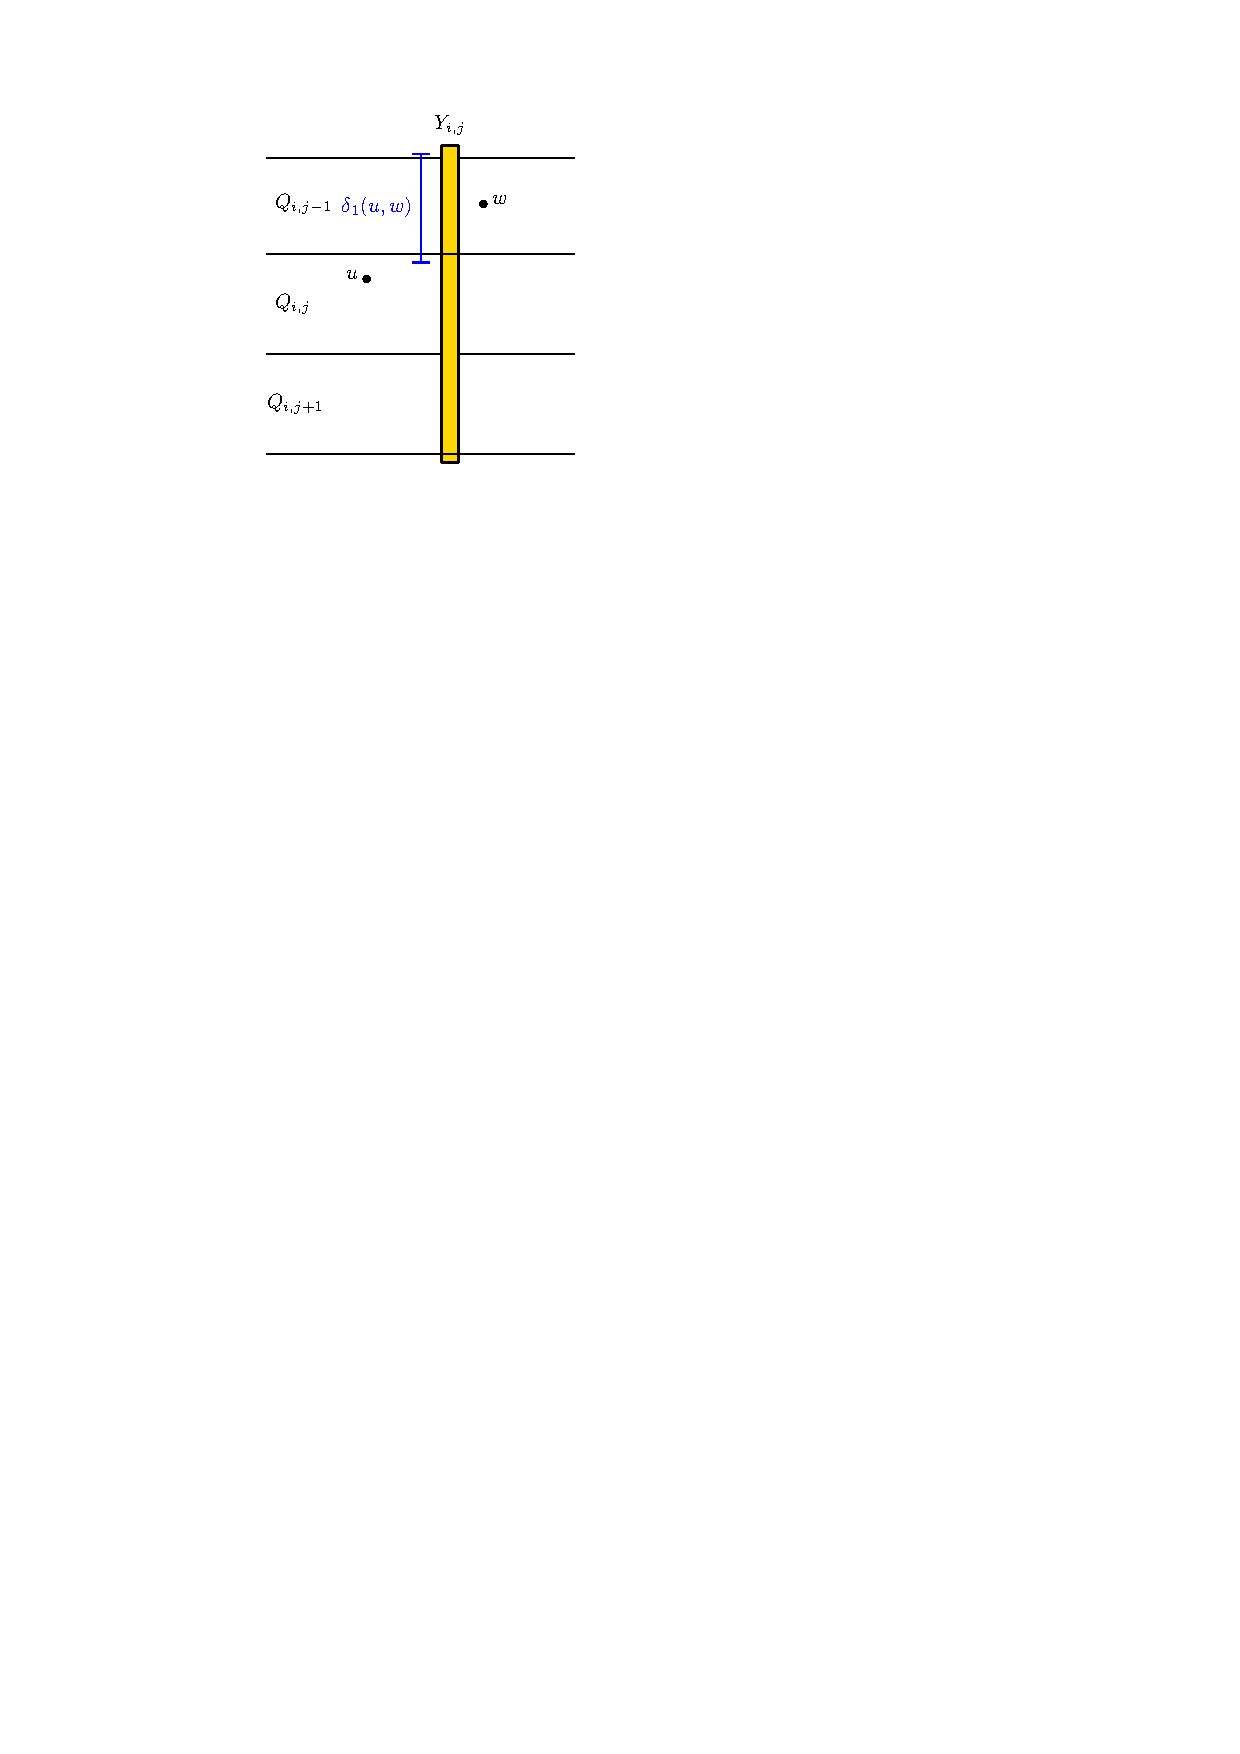
\includegraphics[page=1]{figs/new_metric} &
    \includegraphics[page=2]{figs/new_metric} &
    \includegraphics[page=3]{figs/new_metric}
    \end{tabular}
    \caption{The definitions of $\delta_1$, $\delta_2$, and $\delta_3$.}
\end{figure}

Let $v:=(x_2,y_b)$.  Let $i$ be the maximum integer such that $v$ and $w$ are in $G_{i,j}$ but $v$ and $w$ are in different components of $G_{i,j}-X_{i,j+1}$.  If no such $i$ exists, then define $\delta_2(v,w)=0$.  Otherwise,  $\delta_2(v,w)=a-j2^i + b-j2^i$.

Symmetrically, let $i$ be the maximum integer such that $v$ and $w$ are in $G_{i,j}$ but $v$ and $w$ are in different components of $G_{i,j}-X_{i,j-1}$.  If no such $i$ exists, then define $\delta_2(v,w)=0$.  Otherwise,  $\delta_2(v,w)=(j+1)2^i-a + (j+1)2^i-b$.

Finally, define
\[   d^*(v,w) := \max\{\delta_1(u,w), \delta_2(u,w), \]

\begin{lem}
  The function $d^*:V(H\boxtimes P)\setminus X\to\N$ is a distance function for $V(H\boxtimes P)\setminus X$.
\end{lem}

\begin{proof}
  It is straightforward to verify that $d^*(u,u)=0$ for all $u\in V(H\boxtimes P)\setminus X$ and that $d^(u,v)=d^*(v,u)\ge 0$ for all $u,v\in V(H\boxtimes P)\setminus X$.

  Let $u:=(x_1,y_a)$, $v:=(x_2,y_b)$ and $w:=(x_3,y_c)$ be three vertices of $(H\boxtimes P)- X$.
  % Since $u\not\in X$, $u$ is a vertex of $G_{0,a}$. Therefore $i^*(u,u)=-\infty$, so $d^*(u,u)=2^{-\infty}=0$.
  %
  % Let $v:=(x_2,y_b)\in V(H\boxtimes P)\setminus (X\cup\{u\})$.  Then, since $i^*(v,w)\in \Z\cup \{-\infty\}$, $d^*(u,v)=2^{i^*(u,v)}\ge 0$.  Furthermore, by the definition of $i^*$, $i^*(u,v)=i^*(v,u)$, so $d^*(u,v)=2^{i^*(u,v)}=d^*(v,u)$.
  %
  % Let $w:=(x_2,y_c)\in V(H\boxtimes P)\setminus X$.
  We must show that $d^*(u,w)\le d^*(u,v)+d^*(v,w)$.  If $d^*(u,w)=0$ then this is immediate, so suppose $d^*(u,w)>0$.   If $d^*(u,w)=d_{H\boxtimes P}(u,w)$ then this follows immediately from the fact that $d_{H\boxtimes P}$ satisfies the triangle inequality and $d^*(u,v) + d^*(v,w)\ge d_{H\boxtimes P}(u,v)+d_{H\boxtimes P}(v,w)$.

  Next we consider the case where $d^*(u,w)=\delta_1(u,w)$.
  In this case $i^*(u,w)\ge 0$ and assume, without loss of generality that $i:=i^*(u,w)=\overrightarrow\imath^*(u,w)$.  Let $j:=\floor{a/2^i}$.  Since $w\not\in X$, one of the two cases must occur:
  \begin{compactenum}
    \item $u$ and $w$ are in different components, $C_u$ and $C_w$ of $Q^+_{i,\floor{a/2^i}}-\bigcup_{p=i}^{\log N} X_{i,\lfloor a/2^p\rfloor}$.  We distinguish between two cases depending on the location of $v$.
    \begin{compactenum}
      \item $v\in V(Q^+_{i,j})$.  In this case, $v$ is contained in some component $C_v$ of $Q^+_{i,\floor{a/2^i}}-\bigcup_{p=i}^{\log N} X_{i,\lfloor a/2^p\rfloor}$.  If $C_v\neq C_u$ then $i^*(u,v)\ge i$ so $d^*(u,v)\ge 2^i$ and there is nothing to prove.  If $C_v=C_u$ then we argue that $d_{H\boxtimes P}(u,v)+\delta_s(u,v)\ge 2^i=d^*(u,w)$.
      \item $v\not\in V(Q^+_{i,j})$.  In this case no component of $Q^+_{i,\floor{a/2^i}}-\bigcup_{p=i}^{\log N} X_{i,\lfloor a/2^p\rfloor}$ contains $v$, so $i^*(u,v)\ge i$ and we are also done.
    \end{compactenum}
    \item $w\not\in V(Q^+_{i,j})$.  In this case $d(u,w)\ge 2^i$.
  \end{compactenum}
\end{proof}

The following lemma shows that the metric space $(V(G),d^*)$ has local density at most $3D$:

\begin{lem}
  The metric space $(V(G),d^*)$ has local density at most $3D$.
  % For each $v\in V(H\boxtimes P)$ and $r\ge 0$,
  % $|B_{(V(G),d^*)}(v,r)| \le 3Dr$ \enspace .
\end{lem}

\begin{proof}
  We will only make use of the lower bound $d^*(v,w)\ge \delta_1(v,w)$.
  Since $\delta_1(v,w)$ is always an integer power of $2$, we may assume that $r=2^k$ for some integer $k$.  If $\delta_1(v,w)\le r$ for some $w\in V(G)$, then $v$ and $w$ are in the same component of $Q^+_{i,j}-X_{i,j}$ for some $i \le k$.  For each $i\in\{0,\ldots,k\}$, there are three values of $j$ such that $v\in V(Q^+_{i,j})$.  For each of these, the component of $Q^+_{i,j}-X_{i,j}$ that contains $v$ has at most $D2^{i-1}$ vertices of $G$. Therefore,
  \[
    |B_{(V(G),d^*)}| \le |\{w\in V(G): \delta_1(v,w)\le r\}| \le \sum_{i=0}^{k-1} 3D2^{i} = 3D(2^{k}-1) < 3Dr \enspace . \qedhere
  \]
\end{proof}

\begin{lem}
    The metric space $(V((H\boxtimes P)-X),d^*)$ is a contraction of $(V((H\boxtimes P)-X),d_{(H\boxtimes P)-X})$.
\end{lem}



% \pat{There's a huge hole here that I noticed while writing introductory material.   We need a volume-preserving embedding of $H\boxtimes P-Z$, since that's the metric space with small local density.\\[2ex] I think I know what to do, but this just got a lot more interesting.}


% Since a number of other minor-closed and non-minor-closed graph classes have a product stucture similar to that of planar graphs, we will prove the following result, which generalizes \cref{rao} from planar graphs to product structured graphs.

Note that, although the definition of volume-preserving contractions applies to a metric space $(S,d)$, it is still meaningful when applied to any pair $(S,d^*)$ where $d^*:S^2\to\R_{\ge 0}$ satisfies the requirements of a distance function except, possibly, the triangle inequality.  In this section we will prove the following result:

% \begin{thm}\label{product_contraction}
%   Let $H$ be a graph of treewidth $t\ge 1$, let $P$ be a path, and let $G$ be an $n$-vertex subgraph of $H\boxtimes P$.  Let $G_{i,j}, $Q_{i,j}$, $X_{i,j}$ and $d^*$ be defined as in the previous section (in terms of $H$, $P$, and $G$).  Then $(V(H\boxtimes P), d^*)$ has a $(k,O(t\sqrt{\log n}))$-volume-preserving Euclidean contraction.
% \end{thm}

The proof of \cref{product_contraction} uses many of the ideas from the proof of \cref{rao} given by \citet{rao:small}.

% \david{This suggests we are claiming a version of \cref{fan_partition_planar} for any $n$-vertex subgraph of $H\boxtimes P$ where $H$ has no $K_t$ minor. But the sparsification step requires that $H$ has treewidth less than $t$. We should state the following theorem, including the correct dependence on $t$:

% \begin{thm}\label{fan_partition_HP}
% For every graph $H$ of treewidth $t$ and for every path $P$, every $n$-vertex  subgraph $G$ of $H\boxtimes P$ contains a set $X$ of $O(\sqrt{n}\log^2 n)$ vertices such that $G-X$ has bandwidth $O(\sqrt{n}\log^2 n)$.
% \end{thm}
% }

% The proof of \cref{product_contraction} closely follows Rao's proof of \cref{rao}.




\subsection{Decomposing $H$: The Klein-Plotkin-Rao Partition}

First, fix some integer $\Delta \ge 1$.
Consider the following random process that, given a connected graph $H$ constructs a random subset $\textsc{Chop}_{\Delta,t}(H)$ of vertices in $H$. If $t=0$ then $\textsc{Chop}_{\Delta,0}(H):=\emptyset$.  Otherwise, select any vertex $x$ in $H$ and choose a uniformly random $r\in\{0,\ldots,\Delta-1\}$.  Let $R:=\{y\in V(H):d_{H}(x,y)\equiv r\pmod{\Delta}\}$ and let $C_1,\ldots,C_m$ be the connected components of $H-R$.  Then $\textsc{Chop}_{\Delta,t}(H):=R\cup\bigcup_{i=1}^m \textsc{Chop}_{\Delta,t-1}(C_i)$.


The following lemma, with a greater dependence on $t$, is due to \citet{klein.plotkin.ea:excluded}. The version shown here was proved by \citet{fakcharoenphol.talwar:improved}. The presentation here closely follows that of \citet{lee:simpler}.

\begin{lem}[{\citet{klein.plotkin.ea:excluded,fakcharoenphol.talwar:improved}}]\label{component_diameter_h}
  If $H$ is a connected $K_{t+1}$-minor-free graph, then each component of $H-\textsc{Chop}_{\Delta,t}(H)$ has diameter at most $?t\Delta$.
\end{lem}


% Say that a vertex $x$ of $H$ is \defin{$\delta$-good} with respect to a set $X\substeq V(H)$ if $d_{H}(x,X)\ge \delta$ and $x$ is \defin{$\delta$-bad} with respect to $X$ otherwise.

\begin{lem}\label{delta_bad_h}
  For any vertex $x$ of $H$ and any integer $\delta\ge 1$, $\Pr(d_H(x, \textsc{Chop}_{\Delta,t}(H)< \delta)\le t\,(2\delta-1)/\Delta$.
\end{lem}

\begin{proof}
  The proof is by induction on $t$.
  If $d_H(x,\textsc{Chop}_{\Delta,t}(H) < \delta)$ then $d(x,R)< \delta$ or, if $t>1$,  $d_H(x,\textsc{Chop}_{\Delta,t-1}(C) < \delta)$ where $C$ is the component of $H-R$ that contains $x$.  Since there are at most $2\delta-1$ choices of $r$ for which $d_H(x,R)<\delta$, $\Pr(d_H(x,R)<\delta) \le (2\delta-1)/\Delta$. For $t=1$, this completes the proof.  For $t>1$, the proof follows from the inductive hypothesis on $\textsc{Chop}_{\Delta,t-1}(C)$ and the union bound.
\end{proof}

\subsection{\boldmath Decomposing $Q_{i,j}-X_{i,j}$}

Let $C$ be a component of $Q_{i,j}-X_{i,j}$ for some $i\ge 1$ and some $j$.  Then $C=H'\boxtimes P_{i,j}$ where $H'$ is a subgraph of $H$ (a component of $H-X'_{i,j}$) and $P_{i,j}=y_{(i-1)2^i+1},\ldots,y_{(i+1)2^i}$ is a subpath of $P$ with $3\cdot2^i$ vertices.  Choose a uniformly random $r_0\in\{0,\ldots,\Delta-1\}$, let $A_0:=\{y_{(i-1+a)2^i+1+r_0}: a\in\{0,1,2\}\}$ and let $A:=A(C):=V(H')\times A_0$.  Let $P_1,P_2,P_3$ be the components (each of which is a path) of $P-Y_0$ and let $B_1,B_2,B_3$ be the results of independent executions of $\textsc{Chop}_{2^i,t}(H')$ and let $B:=B(C):=\bigcup_{i=1}^3 V(P_i)\times B_i$.  Finally, let $Z:=Z(C):=B\cup Y$.

% For some intuition, it is helpful to consider the case when $H$ is a path and $t=1$.  In this case, $H\boxtimes P$ is a grid with diagonal edges.  Starting from row $r\in\{0,\ldots,\Delta-1\}$, the set $Y$ contains one out of every $\Delta$ rows of this grid.  Each of the components $C_1,\ldots,C_m$ of $H\boxtimes P-Y$, except the top-most, $C_1$ and bottom-most, $C_m$ is a grid with $\Delta-1$ rows.  For each component $C_i$, the set $X$ contains one out of every $\Delta$ columns of $C_i$, starting from column $r_i\in\{0,\ldots,\Delta-1\}$. \todo{Add figure}

\begin{lem}\label{component_diameter}
  Each component of $C-Z$ has diameter at most $?t2^i$.
\end{lem}

\begin{proof}
  Let $C'$ be a component of $C-Z$.  For any two vertices $x:=(x_1,x_2)$ and $y:=(y_1,y_2)$ of $C'$, $d_{C}(x,y) = \max\{d_{H'-B_j}(x_1,y_1),d_{P'}(x_2,y_2)$ where $B_j$ is the result of running $\textsc{Chop}_{\Delta,t}(H')$. By \cref{component_diameter_h},  $d_{H-X_j}(x_1,y_1)\le ?t\Delta$.  By the choice of $Y_0$, $d_{P}(x,y)<\Delta$.
\end{proof}



\begin{lem}\label{delta_bad_product}
  For any vertex $x$ of $C$ and any integer $\delta\ge 1$, $\Pr(d_{C}(x,Z)< \delta)\le (t+1)(2\delta-1)/\Delta$.
\end{lem}

\begin{proof}
  If $d_{C}(x,Z)<\delta$ then $d_{C}(x,A)<\delta$ or $d_{C}(x,B)<\delta$ where $C$ is the component of $H\boxtimes P-Y$ that contains $x$.  Again, there are at most $2\delta-1$ choices of $r_0$ for which $d_{C}(x,A)<\delta$, so $\Pr(d_{C}(x,A)<\delta)\le (2\delta-1)/\Delta$.  The proof now follows from the union bound and \cref{delta_bad_h}.
\end{proof}

% \Cref{delta_bad_product} with $\delta=1$ yields the following results:
%
% \begin{cor}
%   For any $x\in V(H\boxtimes P)$, $\Pr(x\in Z)\le (t+1)/\Delta$.
% \end{cor}
%
% I don't think this is relevant.

\subsection{\boldmath The Mapping $\phi$}

Let $Z:=Z_{\Delta,t}(H,P)$ a subset of $V(H\boxtimes P)$ generated by running the procedure described above.  Consider the graph $I:=\mathdefin{I(H,P,Z)}$ obtained from $H\boxtimes P$ by removing all edges incident to at least one vertex in $Z$. Let $C_1,\ldots,C_p$ be the components of $I$ and let $\alpha_1,\ldots,\alpha_p$ be mutually independent uniform real numbers in $[0,1]$ and let $\varphi_Z(x):=(1+\alpha_i)\,d^+_{H\boxtimes P}(x,Z)$, for each $x\in C_i$ and each $i\in\{1,\ldots,p\}$.  (Note that this definition uses positive distance $d^+_{H\boxtimes P}$.)

\begin{lem}\label{double_distance}
  For any two vertices $x$ and $y$, $|\varphi_Z(x)-\varphi_Z(y)|\le 2d_{H\boxtimes P}(x,y)$.
\end{lem}

\begin{proof}
  For brevity, let $d(\cdot,\cdot):=d_{H\boxtimes P}(\cdot,\cdot)$ and $d^+(\cdot,\cdot):=d^+_{H\boxtimes P}(\cdot,\cdot)$ throughout this proof.
  Since $1+\alpha_i\le 2$ for all $i$, it suffices to show that $|d^+(x,Y)-d^+(y,Z)|\le d(x,y)$.  If neither $x$ nor $y$ are in $Z$ then $d^+(x,Z)=d(x,Z)$ and $d^+(y,Z)=d(y,Z)$.  Then, by triangle inequality, $d^+(x,Z)-d^+(y,Z)\le d(x,y)$ and $d^+(y,Z)-d^+(x,Z)\le d(x,y)$.

  If exactly one of $x$ or $y$ is in $Z$, say $x$, then $d^+(x,Z)=1=d(y,Z)+1$ and $d^+(y,Z)=d(y,Z)$.  Then $d^+(x,Z)-d^+(y,Z)=1-d^+(y,Z)\le 0$ and, by triangle inequality $d^+(y,Z)-d^+(x,Z)=d(y,Z)-d(x,Z)-1 \le d(x,y)-1< d(x,y)$.

  Finally, if both $x$ and $y$ are in $Z$ then $|d^+(x,Z)-d^+(y,Z)|=0\le d(x,y)$.
\end{proof}


\begin{obs}\label{uniform}
  For any vertex $x$ of $H\boxtimes P$, $\varphi_Z(x)$ is uniformly distributed in the real interval $[d^+_{H\boxtimes P}(x,Z), 2d^+_{H\boxtimes P}(x,Z)]$.
\end{obs}

% The following observation follows immediately from \cref{component_diameter}.  (The $\Delta=1$ case is due to the fact that )
% \begin{obs}\label{independent}
%   Let $x_1,\ldots,x_i$ be distinct vertices $V(H\boxtimes P)$.  If $\Delta=1$ or $d_{H\boxtimes P}(x_i,\{x_1,\ldots,x_{i-1}\})> ?t\Delta$ then the location of $\varphi_Z(x_i)$ in the interval $[d^+_{H\boxtimes P}(x_i,Z), 2d^+_{H\boxtimes P}(x_i,Z)]$ is independent of $\varphi_Z(x_1),\ldots,\varphi_Z(x_{i-1})$.
% \end{obs}

Let $a$ be a constant whose value will be lower-bounded later.  We now define a random function $\phi:V(G)\to\R^{L}$ where $L:=\lfloor 1+\log_2 n\rfloor\cdot\lceil a k\ln n\rceil$. For each $i\in\{0,\ldots,\lfloor \log_2 n\rfloor\}$ and each $j\in\{1,\ldots,\lceil a k\ln n\rceil\}$, let $Z_{i,j}\sim Z_{\Delta,t}(H,P)$ be the random subset of $V(H\boxtimes P)$ obtained by using the procedure described above with parameters $\Delta=2^i$ and $t$ with all random choices made independently.  For each $x\in V(H\boxtimes P)$, let $\phi_{i,j}(x):= \varphi_{Z_{i,j}}(x)$ again with all choices made independently.  Finally,
\[
   \phi(x) := \left(\phi_{i,j}(x):(i,j)\in \{0,\ldots,\lfloor \log_2 n\rfloor\}\times\{1,\ldots,\lceil a k\ln n\rceil\}\right) \enspace .
\]
Although $\phi$ maps vertices of $H\boxtimes P$ to $\R^L$, it is not necessarily a Euclidean contraction: $\phi$ has $L$ coordinates and for two vertices $x$ and $y$, the difference between $\phi_{i,j}(x)$ and $\phi_{i,j}(y)$ can be as much as $2d_{H\boxtimes P}(x,y)$ (but not more).  Thus, $d_2(\phi(x),\phi(y))$ can exceed $d_{H\boxtimes P}(x,y)$ by a factor of up to $2\sqrt{L}$ (but not more).  In a final step, we will divide each coordinate of $\phi$ by $2\sqrt{L}$ but, until then, it is more convenient to work with $\phi$.

The rest of the analysis in this section closely follows \citet{rao:small}, which in turn closely follows \citet{feige:approximating} with modifications needed to work in the metric $(V(G),d_{H\boxtimes P})$.  Nevertheless, we proceed slowly and carefully since our setting is significantly different (we are working in a subgraph $G$ of $H\boxtimes P$ but using the metric space $(V(G),d_{H\boxtimes P})$) and we expect that some readers will not be familiar with some methods introduced by \citet{feige:approximating} that are only sketched by \citet{rao:small}.

We make use of this simple \defin{Chernoff Bound}: For a $\operatorname{binomial}(n,p)$ random variable $B$ and any $0<\delta<1$, $\Pr(B \le np/2) \le \exp(-np/8)$.

Let $\Gamma_k:=\{(\lambda_1,\ldots,\lambda_k)\in \R^k:\sum_{j=1}^k\lambda_j=1\}$, that is, $\Gamma_k$ is the set of coefficients that can be used to obtain an affine combination of $k$ items.


\begin{lem}\label{crux}
  Fix some function $\lambda:(\R^{L})^{p-1}\to \Gamma_{p-1}$. Let $H$ be $K_{t+1}$-minor-free graph with at most $n$ vertices, let $P$ be a path with at most $n$ vertices, and let $\phi:V(H\boxtimes P)\to\R^L$ be the probabilistic embedding defined above. In particular, the random choices made in the construction of $\phi$ are independent of $\lambda$.  Let $v_1,\ldots,v_p$ be distinct vertices of $H\boxtimes P$ and let $h:=d_{H\boxtimes p}(v_p,\{v_1,\ldots,v_{p-1}\})$.  Let $(\lambda_1,\ldots,\lambda_{p-1}):=\lambda(\phi(v_1),\ldots,\phi(v_{p-1}))$ and let $x:=\sum_{j=1}^{p-1}\lambda_j\phi(v_j)$.
  Then, with probability at least $1-n^{-3k}$,
  \[
    d_2(\phi(v_p),x)\ge \frac{h\sqrt{ak\ln n}}{160?(t+1)} \enspace
  . \]
\end{lem}

\begin{proof}
  If $h <?$ then let $i:=0$.  Otherwise, let $i$ be the unique (positive) integer such that $h/2?< 2^i \le h/?$, where $?$ is the constant in \cref{component_diameter_h} and let $\Delta=2^i$.  We will focus on the coordinates $\phi_{i,1},\ldots,\phi_{i,\lceil a k\ln n\rceil}$.  We say that $j\in\{1,\ldots,\lceil a k\ln n\rceil\}$ is \defin{good} if $d_{H\boxtimes P}(v_p,Z_{i,j})\ge \Delta/10(t+1)$.  By \cref{delta_bad_product},  $\Pr(\text{$j$ is good})\ge 1-(t+1)(2\Delta/10(t+1)-1)/\Delta > 3/5$. Let $J:=\{j\in\{1,\ldots,\lceil a k\ln n\rceil\}:\text{$j$ is good}\}$.  Since $Z_{i,1},\ldots,Z_{i,\lceil a k\ln n\rceil}$ are mutually independent, $|J|$ dominates\footnote{We say that a random variable $X$ \defin{dominates} a random variable $Y$ if $\Pr(X\ge x)\ge\Pr(Y\ge x)$ for all $x\in\R$.} a $\operatorname{binomial}(\lceil a k\ln n\rceil,3/5)$ random variable. By the Chernoff Bound, $\Pr(|J|\ge \tfrac{3}{10}\lceil a k\ln n\rceil)\ge 1-\exp(-3ak\ln n/80)$.

  By \cref{uniform} $\phi_{i,j}(v_p)$ is uniformly distributed over an interval of length at least $\Delta/10(t+1)$, for each $j\in J$.  We claim that the location of $\phi_{i,j}(v_p)$ in this interval is independent of the corresponding coordinate, $x_{i,j}$, of $x$.
  Since $d_{H\boxtimes P}(v_p,\{v_1,\ldots,v_{p-1}\})= h$, either $\Delta=1$ or \cref{component_diameter} implies that the component of $(H\boxtimes P)-Z$ that contains $v_p$ does not contain any of $v_1,\ldots,v_{p-1}$. In either case, the component of $I(H,P,Z_{i,j})$ that contains $v_p$ does not contain any of $v_1,\ldots,v_{p-1}$.  Therefore, the location of $\phi_{i,j}(v_p)$ is determined by a random real number $\alpha\in[0,1]$ that does not contribute to $\phi(v_1),\ldots,\phi(v_{p-1})$.  Since $(\lambda_1,\ldots,\lambda_{p-1})=\lambda(\phi(v_1),\ldots,\phi(v_{p-1}))$ is completely determined by $\phi(v_1),\ldots,\phi(v_{p-1})$, $\alpha$ is independent of $x=\sum_{k=1}^{p-1}\lambda_k\phi(v_k)$.  In particular, $\alpha$ is independent of $x_{i,j}$.

  Therefore, for $j\in J$, $\Pr(|\phi_{i,j}(v_p)-x_{i,j}|\ge \Delta/40(t+1))\ge 1/2$.\footnote{The coordinate $\phi_{i,j}(v_p)$ is uniform over some interval $[a,b]$ of length $b-a\ge \Delta/10(t+1)$ whereas $[x_{i,j}-\Delta/40(t+1),x_{i,j}+\Delta/40(t+1)]$ has length $\Delta/20(t+1)$, so $\Pr(|\phi_{i,j}(v_p)-x_{i,j}|\ge \Delta/40(t+1))\ge (b-a-\Delta/20(t+1))/(b-a)\ge 1/2$.}
  Let $J':=\{j\in J:  |\phi_{i,j}(v_p)-x_{i,j}|\ge \Delta/40(t+1)\}$.  Then $|J'|$ dominates a $\operatorname{binomial}(|J|,1/2)$ random variable.  By the Chernoff Bound (and the union bound), $\Pr(|J'|\ge \tfrac{3}{40}\lceil a k\ln n\rceil)\ge 1-\exp(-3ak\ln n/160)-\exp(-3ak\ln n/80)\ge 1-n^{-3k}$ for all $a\ge 500$, $n\ge 2$, and $k\ge 2$. Therefore,
  \begin{align*}
    d_2(\phi(v_p),x)
    & = \left(\sum_{i'=0}^{\lfloor\log_2 n\rfloor}\sum_{j=1}^{\lceil ak\ln  n\rceil}(\phi_{i',j}(v_p)-x_{i',j})^2\right)^{1/2} \\
    & \ge \left(\sum_{j=1}^{\lceil ak\ln  n\rceil}(\phi_{i,j}(v_p)-x_{i,j})^2\right)^{1/2} \\
    & \ge \left(\sum_{j\in J'}(\Delta/40(t+1))^2\right)^{1/2} \\
    & \ge \left((\Delta/40(t+1))^2\cdot \tfrac{1}{4}\lceil ak\ln  n\rceil\right)^{1/2}
      & \text{(with probability at least $1-n^{-3k}$)} \\
    & = \frac{\Delta\sqrt{\lceil ak\ln  n\rceil}}{80(t+1)} \\
    & \ge \frac{h\sqrt{\lceil ak\ln n\rceil}}{160?(t+1)}
     & \text{(since $\Delta\ge h/2?$)}. &
    \qedhere
  \end{align*}
\end{proof}

\begin{lem}\label{volume_preserver}
  Let $H$ be $K_{t+1}$-minor-free graph with at most $n$ vertices, let $P$ be a path with at most $n$ vertices, and let $\phi:V(H\boxtimes P)\to\R^L$ be the probablistic embedding defined above.  Then, for any $k$-element subset $K$ of $V(H\boxtimes P)$,
  \[
    \Pr\left(\evol(\phi(K)) \ge \frac{\tvol_{d_{H\boxtimes P}}(K)\cdot(2\zeta/3)^{k-1}}{(k-1)!}\right) \ge 1- O(kn^{-k}) \enspace .
  \]
  where $\zeta:=\sqrt{\lceil ak\ln n\rceil}/160?(t+1)$ is the expression that also appears in \cref{crux}.
\end{lem}

\begin{proof}
  The following argument is due to \citet[Pages~529--530]{feige:approximating}.  Let $K$ be a set of $k$ vertices of $G$.  Let $T$ be a minimum spanning tree of the complete graph on $K$ where the weight of an edge $xy$ is $d_{H\boxtimes P}(x,y)$.  Let $x_1,\ldots,x_k$ be an ordering of the vertices in $K$ and $T_1,\ldots,T_k$ be a sequence of trees such that $T_{p}$ is a minimum spanning tree of $x_1,\ldots,x_{p}$ that contains $T_{p-1}$ as a subgraph, for each $p\in\{2,\ldots,k\}$.  That such an ordering and sequence of trees exists follows from the correctness of Prim's Algorithm. For each $p\in\{2,\ldots,k\}$, let $h_p:=d_{H\boxtimes P}(x_p,\{x_1,\ldots,x_{p-1}\})$ be the cost of the unique edge in $E(T_p)\setminus E(T_{p-1})$.  Observe that $\prod_{p=2}^k h_p = \tvol_{d_{H\boxtimes P}}(K)$.

  For each $p\in\{2,\ldots,k\}$, let $B_{p-1}:=\left\{\sum_{i=1}^{p-1}\lambda_i\phi(v_i):(\lambda_1,\ldots,\lambda_{p-1})\in\Gamma_{p-1}\right\}$ be the subspace of $\R^L$ spanned by $\phi(v_1),\ldots,\phi(v_{p-1})$.  Then
  \[
    \evol(\{v_1,\ldots,v_p\})=\evol(\{v_1,\ldots,v_{p-1}\}\cdot d_2(v_p,B_{p-1})/(p-1))\enspace .\footnotemark
  \]
  \footnotetext{This is the $(p-1)$-dimensional generalization of the formula $a:=bh/2$ for the area $a$ of a triangle $v_1,v_2,v_3$ with base length $b=\evol(\{v_1,v_2\})$ and height $h=d_2(v_3,B_2)$, where $B_2$ is the line containing $v_1$ and $v_2$.}  Observe that each coordinate $\phi_{i,j}(v_p)$ of $\phi(v_p)$ is at most $2(n-1)$, since $\phi_{i,j}(v_p)=\alpha_{Z_{i,j}}(v_p)\cdot d_{H\boxtimes P}(v_p, Z_{i,j})\le 2(n-1)$. Therefore, $\phi(v_p)$ is contained in a ball $B$ of radius $2(n-1)\sqrt{L}$ around the origin. \citet{feige:approximating} uses these two facts to show $Q_{p-1}\cap B$ can be covered by $\Theta(n^{2k})$ balls, each of radius $h\zeta$, such that, if $\phi(v_p)$ is not contained in any of these balls, then $d_2(\phi(v_p),Q_{p-1})\ge 2q\zeta/3$.  When this happens,
  \[
    \evol(\{\phi(v_1),\ldots,\phi(v_p)\})\ge (2q\zeta/3)\cdot\evol(\{\phi(v_1),\ldots,\phi(v_{p-1})\})/(p-1).
  \]
  By \cref{crux}, the probability that $\phi(p)$ is not contained in any of these balls is at least $1-O(n^{-k})$. By the union bound, the probability that this occurs for each $p\in\{2,\ldots,k\}$ is at least $1-O(kn^{-k})$.  Therefore, with probability at least $1-O(kn^{-k})$,
  \[
    \evol(\phi(K)) \ge \prod_{p=2}^{k}\frac{h_p(2\zeta/3)}{p-1} = \frac{\tvol_{d_{H\boxtimes P}(K)}(2\zeta/3)^{k-1}}{(k-1)!} \enspace . \qedhere
  \]
\end{proof}

We now have all the pieces needed to complete the proof of \cref{product_contraction}.

\begin{proof}[Proof of \cref{product_contraction}]
  For each $v\in V(H\boxtimes P)$, let $\phi'(p):=\phi(p)/2\sqrt{L}$, so that $\phi'$ is a Euclidean contraction of $(V(H\boxtimes P),d_{H\boxtimes P})$.  By \cref{volume_preserver}, for each $K\in \binom{V(G)}{k}$,
  \begin{equation}
    \Pr\left(\evol(\phi'(K)) \ge \frac{\tvol_{d_{H\boxtimes P}}(K)\cdot(2\zeta/3)^{k-1}}{(k-1)!(2\sqrt{L})^{k-1}}\right) \ge 1- O(kn^{-k}) \enspace .
    \label{zippy}
  \end{equation}
  By the union bound, the probability that the volume bound in \cref{zippy} holds for every $K\in\binom{V(G)}{k}$ is at least $1-O(\binom{n}{k}kn^{-k}) > 0$ for sufficiently large $n$.  When this occurs,
  \[
    \evol(\phi'(K)) \ge \frac{\tvol_{d_{H\boxtimes P}}(K)\cdot(2\zeta/3)^{k-1}}{(k-1)!(2\sqrt{L})^{k-1}} \ge
    \frac{\ivol_{d_{H\boxtimes P}}(K)\cdot(2\zeta/3)^{k-1}}{(2\sqrt{L})^{k-1}} \enspace ,
  \]
  so $\phi'$ is a $(k,\eta)$-volume-preserving contraction for
  \[
    \eta = \frac{2\sqrt{L}}{\zeta} = \frac{160?(t+1)2\sqrt{L}}{\sqrt{\lceil ak\ln n\rceil}} = {160?(t+1)2\sqrt{1+\log_2 n}} = O(t\sqrt{\log n}) \enspace . \qedhere
  \]
\end{proof}

The proof of \cref{main_thm_products} is exactly the same as the proof of \cref{main_thm_planar} except that we use the $(k,O(\sqrt{\log n}))$-volume-preserving contraction guaranteed by \cref{product_contraction} instead of the one guaranteed by \cref{rao}.

\section{Discussion}

For fixed $t\ge 3$, the $O(\sqrt{\log n})$ bound in \cref{product_contraction} is tight, since it is already tight for planar graphs, even for $k=1$ \cite{?}.

\Cref{product_contraction} extends easily to any $n$-vertex subgraph $G$ of $H\boxtimes P\boxtimes P\boxtimes\cdots\boxtimes P$ where $H$ is $K_{t+1}$-minor-free and $P$ appears $s$ times in the product.  In this case, one obtains a $(k,O(st\sqrt{\log n}))$-volume-preserving Euclidean contractions of $(V(G),d_{H\boxtimes P\boxtimes P\cdots\boxtimes P})$.

\begin{tcolorbox}[width=\textwidth,colback={orange}]
  One direction for future work is to look at the algorithmic results in \citet{klein.plotkin.ea:excluded} and see if they can be extended to subgraphs of $H\boxtimes P\boxtimes\cdots\boxtimes P$.  This paper seems to be quite influential and I think the decomposition is used in a bunch of other problems.  Here's a starting point:

  \begin{thm}
    Let $G$ be an $n$-vertex subgraph of $H\boxtimes P\boxtimes\cdots\boxtimes P$ where $H$ is $K_{t+1}$-minor-free and $P$ appears $s$ times in the product.  Then for every number $\Delta\ge 1$ there exists a partition $\mathcal{P}$ of $V(H\boxtimes P\boxtimes \cdots\boxtimes P)$ such that
    \begin{compactenum}[(i)]
      \item For each part $P\in\mathcal{P}$, $(H\boxtimes P\boxtimes \cdots\boxtimes P)[P]$ has diameter $O(t\Delta)$; and
      \item the number of edges of $G$ with endpoints in two different parts of $\mathcal{P}$ is $O((t+s)n/\Delta)$.
    \end{compactenum}
  \end{thm}
  The catch, here, is that the diameter of the parts is measured by distances in $H\boxtimes P\boxtimes\cdots\boxtimes P$, not by distances in $G$.  (See, also, the next paragraph.)  I don't know if this is enough to make the algorithmic applications work.
\end{tcolorbox}

Using our methods, \cref{planar_density_bandwidth}, which states that planar graphs of local density $D$ have bandwidth $O(D\log^3 n)$, does not extend to $n$-vertex subgraphs $G$ of  $H\boxtimes P$. This is because the graph metric space $(V(G),d_G)$ can be wildly different than the metric space $(V(G),d_{H\boxtimes P})$. Indeed, any $n$-vertex path $G$ in $H\boxtimes P$ has local density $2$, even if a ball of radius $1$ in $H\boxtimes P$ contains $V(G)$.  Of course, Feige's bound of $O(D\log^3\sqrt{\log n\log\log n})$ still holds for arbitrary graphs.

\todo[inline]{Note that the situation described above never occurs when the mapping of $G$ into $H\boxtimes P$ comes from the existence proof in, e.g., \cite{dujmovic.joret.ea:planar}.  If $G$ has local density $D$ then it has diameter $\Omega(n/D)$, so any BFS layering of $G$ uses $\Omega(n/D)$ layers, so the mapping of $G$ into $H\boxtimes P$ uses a path $P$ with $\Omega(n/D)$ vertices.  This doesn't immediately mean that the metric space $(V(G),d_{H\boxtimes P})$ has local density $O(D)$, but maybe this actually happens for free? Probably not, but maybe it's worth looking into local-density preserving embeddings of graphs into $H\boxtimes P$.}

Open problems:

\begin{itemize}
\item Can the $O(\polylog n)$ factor be removed from \cref{main_thm_planar}? That is, is every $n$-vertex planar graph contained in the $O(\sqrt{n})$-blowup of a fan?

\item Can our results be generalised for arbitrary minor-closed classes? In particular, is every $n$-vertex  graph excluding a fixed minor contained in the $\tilde{O}(\sqrt{n})$-blowup of a fan? It is even open  whether every $n$-vertex graph excluding a fixed minor is contained in the $\tilde{O}(\sqrt{n})$-blowup of a graph with bounded pathwidth (and even if the pathwidth bound is allowed to depend on the excluded minor).  Positive results are known for blowups of bounded treewidth graphs. \citet{distel.dujmovic.ea:product} showed that every $n$-vertex graph excluding a fixed minor is contained in the $O(\sqrt{n})$-blowup of a graph with treewidth 4.
\end{itemize}

\section*{Acknowledgement}

This research was initiated and much of it was done at the \emph{Eleventh Annual Workshop on Geometry and Graphs (WoGaG~2024)} held at the Bellairs Research Institute of McGill University, March 8--15, 2024. The authors are gratefuly to the workshop organizers and other participants for providing a working environment that somehow manages to be simultaneously stimulating and comfortable.

% ?Let $\phi'(x):=\phi(x)/\sqrt{L}$ for each $x\in V(H\boxtimes P)$.

\bibliographystyle{plainurlnat}
\bibliography{fan-partition}

\end{document}
